\documentclass[11pt,a4paper]{article}

\usepackage[a4paper,margin=2.0cm]{geometry}
\usepackage[T1]{fontenc}
\usepackage{lmodern}
\usepackage{microtype}
\usepackage{amsmath,amssymb}
\usepackage{graphicx}
\usepackage{booktabs}
\usepackage{multirow}
\usepackage{array}
\usepackage{float}
\usepackage[font=small,labelfont=bf]{caption}
\usepackage{subcaption}
\usepackage{xcolor}
\usepackage{enumitem}
\usepackage{tikz}
\usetikzlibrary{arrows.meta,positioning,calc}
\usepackage[colorlinks=true,linkcolor=blue!50!black,citecolor=blue!50!black,urlcolor=blue!50!black]{hyperref}

\graphicspath{{./}{../results/figures/}}
\setlist{itemsep=1pt,topsep=3pt}
\setlength{\parskip}{3pt}
\usepackage{tocloft}
\setlength{\cftbeforesecskip}{3pt}

\newcommand{\imf}[1]{\mathrm{IMF}_{#1}}
\newcommand{\snrin}{\mathrm{SNR}_\mathrm{in}}
\newcommand{\snrout}{\mathrm{SNR}_\mathrm{out}}
\newcommand{\snrimp}{\mathrm{SNR}_\mathrm{imp}}

\tikzset{
  blk/.style={draw, rounded corners=2pt, minimum height=6mm, minimum width=15mm,
              font=\footnotesize, align=center, fill=blue!6},
  emd/.style={blk, fill=orange!15, minimum height=14mm},
  sumn/.style={draw, circle, inner sep=0.8pt, font=\footnotesize, fill=white},
  lab/.style={font=\scriptsize, inner sep=1pt},
  >={Latex[length=1.6mm]}
}

\begin{document}

%======================================================================== title
\begin{titlepage}
\centering

\includegraphics[width=3.2cm]{figures/uom_logo.png}\par\vspace{0.5cm}
{\large Department of Electronic and Telecommunication Engineering\\University of Moratuwa, Sri Lanka\par}
\vspace{1.2cm}
{\Large\bfseries BM4152 Biosignal Processing\par}
\vspace{0.3cm}
{\large Final Project Report\par}
\vspace{2cm}
\rule{\linewidth}{0.6pt}\\[0.4cm]
{\LARGE\bfseries Denoising ECG by Adaptive Filtering with\\[0.2cm] Empirical Mode Decomposition\par}
\vspace{0.3cm}
{\large Implementation, Parameter Tuning and Critical Evaluation\par}
\rule{\linewidth}{0.6pt}
\vspace{1.2cm}

{\large Reproduction of: B.~Dai and W.~Bai, \emph{``Denoising ECG by Adaptive Filter with Empirical Mode Decomposition''}~\cite{dai}\par}
\vspace{2.2cm}

{\large\bfseries Group members\par}
\vspace{0.3cm}
\begin{tabular}{ll}
\toprule
Index number & Name \\
\midrule
220472T & Perera P.\,L.\,P. \\
220374U & Madusanka S.\,P.\,S. \\
\bottomrule
\end{tabular}

\vspace{1.5cm}
{\large\bfseries Codebase\par}
\vspace{0.2cm}
{\large \url{https://github.com/LuchithaP/EMD_for_ECG}\par}

\vfill
{\large October 2026\par}
\end{titlepage}

%======================================================================== abstract + toc
{\small\setlength{\parskip}{0pt}\tableofcontents}
\vspace{4mm}\hrule\vspace{2mm}

%======================================================================== 1
\section{Introduction and Background}

ECG recordings are corrupted by four main noises~\cite{moody_nst}: baseline wander (BW, slow drift below about
1\,Hz), power-line interference (PLI, 50/60\,Hz), electrode-motion artefact (EM) and muscle artefact (MA). Notch
and high-pass filters handle PLI and BW. EM and MA share the ECG band, so fixed filters cannot remove them without
also distorting the ECG.

Adaptive noise cancellation~\cite{haykin} uses a reference signal that is correlated with the noise to estimate the
noise and subtract it. Empirical mode decomposition (EMD)~\cite{huang} splits a signal into intrinsic mode functions
(IMFs), ordered from fast to slow. Dai and Bai~\cite{dai} combine the two: each noise's canceller is applied only to
the IMFs that hold that noise. This report describes our implementation, compares our results with the paper's, and
explains where and why they differ.

%======================================================================== 2
\section{Overview of the Selected Paper and Datasets}

\subsection{The paper}
The paper makes two contributions.
\begin{enumerate}
  \item \textbf{BW + PLI removal.} The noisy ECG is decomposed by EMD. An adaptive filter driven by a 60\,Hz reference
        cleans IMF1, and a second filter driven by a BW reference cleans $\imf{5}+\dots+\imf{8}$. IMF2--IMF4 and the
        residue are added back unchanged (Eq.~(1) of~\cite{dai}). LMS, NLMS and RLS cancellers are compared (Fig.~7),
        and EMD+LMS is compared with three published methods (articles [21, 22, 28] of~\cite{dai}) at $\snrin=10$\,dB (Fig.~8).
  \item \textbf{BW + PLI + EM + MA removal.} Two EMD-based structures (PEAF, SEAF) are compared with two direct
        structures (PDAF, SDAF). The paper reports that \emph{PEAF achieves the highest SNR improvement on every
        record and at every input SNR} (Figs.~10, 11).
\end{enumerate}
An IMF selection study (Sec.~III-A) fixes the IMFs used for each noise: PLI $\to$ IMF1, BW $\to$ IMF5--8,
EM $\to$ IMF3--8, and MA $\to$ the whole signal (no EMD).

\subsection{Datasets}
\begin{itemize}
  \item \textbf{MIT-BIH Arrhythmia Database}~\cite{moody_mit,physionet}: 48 two-channel, 30-minute ambulatory
        records sampled at 360\,Hz with 11-bit resolution. We use the MLII lead (channel 0). Fig.~8 uses records
        119, 202, 213, 217 and 234. Figs.~10--11 use records 100, 103, 104, 105, 106, 111, 113, 115, 116, 121, 122, 123
        and 231.
  \item \textbf{MIT-BIH Noise Stress Test Database (NSTDB)}~\cite{moody_nst}: 30-minute recordings of \texttt{bw},
        \texttt{em} and \texttt{ma} noise. They were recorded from an active volunteer with electrodes placed where
        the ECG is not visible, at 360\,Hz. PLI is synthesised as a 60\,Hz sinusoid.
\end{itemize}
Both databases are public on PhysioNet, so we could follow the paper's data choice exactly. The paper does not
publish its code.

%======================================================================== 3
\section{Methods}

\subsection{Empirical mode decomposition}
EMD writes a signal as $x(t)=\sum_{k=1}^{K} c_k(t) + r(t)$, where the $c_k$ are IMFs and $r$ is the residue. Each
IMF is extracted by repeatedly subtracting the mean of the cubic-spline envelopes through the local maxima and
minima (sifting)~\cite{huang}. IMF1 holds the fastest oscillations and the last IMFs the slowest. The method relies on
this ordering.

\subsection{Adaptive noise canceller}
Fig.~\ref{fig:struct}(a) shows the canceller used by every structure. The primary input is
$d(n) = s(n) + v(n)$, where $s(n)$ is the clean ECG and $v(n)$ is the noise. The reference input $u(n)$ is correlated
with $v(n)$. An $L$-tap FIR filter produces the noise estimate $y(n)=\mathbf{w}^{T}(n)\mathbf{u}(n)$, and the error
$e(n)=d(n)-y(n)$ is the denoised output. The LMS update is
\begin{equation}
  \mathbf{w}(n{+}1)=\mathbf{w}(n)+\mu\, e(n)\,\mathbf{u}(n). \label{eq:lms}
\end{equation}
NLMS divides the step by $\|\mathbf{u}(n)\|^2$, and RLS uses a recursive least-squares solution with forgetting factor
$\lambda$~\cite{haykin}. Two LMS properties matter later~\cite{haykin}:
\begin{itemize}
  \item \textbf{Stability:} LMS is stable only for roughly $0<\mu<2/(L\,P_u)$, where $P_u$ is the reference power.
  \item \textbf{Residual error:} the ECG stays in $e(n)$, so a fixed $\mu$ leaves an excess error of about
        $\mathcal{M}P_s$, where $\mathcal{M}\approx\mu LP_u/2$ and $P_s$ is the ECG power.
\end{itemize}

\subsection{IMF selection (Fig.~2 of the paper)}
Each noise is added to the ECG on its own. For every contiguous IMF range $\imf{i}\!\sim\!\imf{j}$
($1\le i\le j\le 8$), and for the whole signal, the canceller is applied to the sum of those IMFs. The other IMFs and
the residue are added back unchanged: $Y = x - \sum_{k=i}^{j} c_k + \mathrm{AF}\big(\sum_{k=i}^{j} c_k\big)$. The
range with the highest $\snrimp$ is selected.

\subsection{Denoising structures}
\textbf{BW + PLI} (Fig.~3, Eq.~(1) of~\cite{dai}):
\begin{equation}
  Y = \imf{1}' + \textstyle\sum_{k=2}^{4}\imf{k} + \imf{58}' + r,
\end{equation}
where $'$ denotes the output of the PLI or BW canceller.

\textbf{PEAF} (parallel EMD adaptive filter, Fig.~\ref{fig:struct}(c)). The BW and EM cancellers run in parallel on
the overlapping ranges IMF5--8 and IMF3--8, and the doubly counted IMF5--8 is subtracted once:
\begin{equation}
  X' = \imf{1}' + \imf{2} + \imf{38}' + \imf{58}' + r - \textstyle\sum_{k=5}^{8}\imf{k}, \qquad Y=\mathrm{AF}_{\mathrm{MA}}(X').
  \label{eq:peaf}
\end{equation}
\textbf{SEAF} (staged EMD adaptive filter, Fig.~\ref{fig:struct}(d)). BW is removed first. The EM canceller then acts
on $\imf{3}+\imf{4}+\imf{58}'$:
\begin{equation}
  X' = \imf{1}' + \imf{2} + \imf{38}'' + r, \qquad Y=\mathrm{AF}_{\mathrm{MA}}(X').
  \label{eq:seaf}
\end{equation}
\textbf{SDAF} (Fig.~\ref{fig:struct}(b)) is the cascade of Thakor and Zhu~\cite{thakor} without EMD, extended with an MA
stage: PLI and BW cancellers in parallel with one shared error, then EM, then MA. \textbf{PDAF} treats all noises as
one and uses a single canceller (Fig.~\ref{fig:struct}(a)) whose reference is the sum of all references.

\begin{figure}[t]
\centering
\begin{subfigure}[b]{0.42\textwidth}
\centering
\resizebox{0.95\textwidth}{!}{%
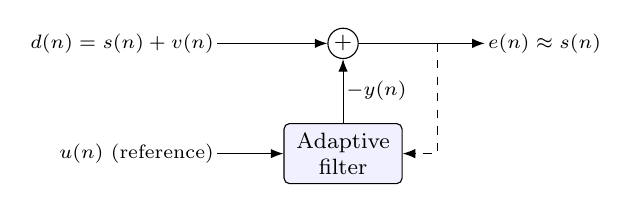
\begin{tikzpicture}
  \node[lab, anchor=east] (d) at (0,0) {$d(n)=s(n)+v(n)$};
  \node[sumn] (s) at (1.6,0) {$+$};
  \node[lab, anchor=west] (o) at (3.4,0) {$e(n)\approx s(n)$};
  \node[lab, anchor=east] (u) at (0,-1.4) {$u(n)$ (reference)};
  \node[blk] (af) at (1.6,-1.4) {Adaptive\\filter};
  \draw[->] (d) -- (s);
  \draw[->] (u) -- (af);
  \draw[->] (af) -- node[lab,right]{$-y(n)$} (s);
  \draw[->] (s) -- (o);
  \draw[->,dashed] (2.8,0) -- (2.8,-1.4) -- (af.east);
\end{tikzpicture}}
\caption{Adaptive noise canceller (Fig.~1 of~\cite{dai})}
\end{subfigure}\hfill
\begin{subfigure}[b]{0.52\textwidth}
\centering
\resizebox{0.95\textwidth}{!}{%
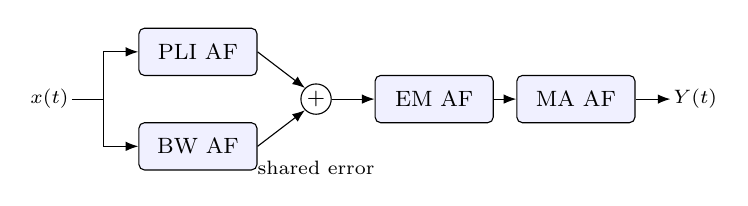
\begin{tikzpicture}
  \node[lab, anchor=east] (x) at (0,0) {$x(t)$};
  \node[blk] (pli) at (1.6,0.6) {PLI AF};
  \node[blk] (bw)  at (1.6,-0.6){BW AF};
  \node[sumn] (s) at (3.1,0) {$+$};
  \node[lab, anchor=north] at (3.1,-0.75) {shared error};
  \node[blk] (em) at (4.6,0) {EM AF};
  \node[blk] (ma) at (6.4,0) {MA AF};
  \node[lab, anchor=west] (y) at (7.6,0) {$Y(t)$};
  \draw (x) -- (0.4,0);
  \draw[->] (0.4,0) |- (pli);
  \draw[->] (0.4,0) |- (bw);
  \draw[->] (pli.east) -- (s.north west);
  \draw[->] (bw.east) -- (s.south west);
  \draw[->] (s) -- (em);
  \draw[->] (em) -- (ma);
  \draw[->] (ma) -- (y);
\end{tikzpicture}}
\caption{SDAF, no EMD (Fig.~5 of~\cite{dai})}
\end{subfigure}

\vspace{4mm}
\begin{subfigure}[b]{0.49\textwidth}
\centering
\resizebox{\textwidth}{!}{%
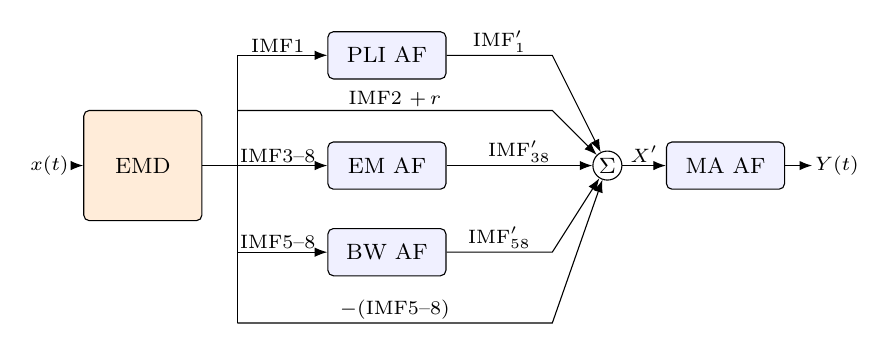
\begin{tikzpicture}
  \node[lab, anchor=east] (x) at (-0.2,0) {$x(t)$};
  \node[emd] (e) at (0.7,0) {EMD};
  \draw[->] (x) -- (e);
  \draw (e.east) -- (1.9,0);
  \draw (1.9,1.4) -- (1.9,-2.0);
  \node[blk] (pli) at (3.8,1.4) {PLI AF};
  \node[blk] (em)  at (3.8,0)   {EM AF};
  \node[blk] (bw)  at (3.8,-1.1){BW AF};
  \node[sumn] (S) at (6.6,0) {$\Sigma$};
  \node[blk] (ma) at (8.1,0) {MA AF};
  \node[lab, anchor=west] (y) at (9.2,0) {$Y(t)$};
  \draw[->] (1.9,1.4) -- node[lab,above,pos=0.45]{IMF1} (pli);
  \draw[->] (1.9,0) -- node[lab,above,pos=0.45]{IMF3--8} (em);
  \draw[->] (1.9,-1.1) -- node[lab,above,pos=0.45]{IMF5--8} (bw);
  \draw[->] (1.9,0.7) -- node[lab,above,pos=0.5]{IMF2 $+\,r$} (5.9,0.7) -- (S);
  \draw[->] (1.9,-2.0) -- node[lab,above,pos=0.5]{$-$(IMF5--8)} (5.9,-2.0) -- (S);
  \draw[->] (pli.east) -- node[lab,above]{IMF$_1'$} (5.9,1.4) -- (S);
  \draw[->] (em.east) -- node[lab,above]{IMF$_{38}'$} (S);
  \draw[->] (bw.east) -- node[lab,above]{IMF$_{58}'$} (5.9,-1.1) -- (S);
  \draw[->] (S) -- node[lab,above]{$X'$} (ma);
  \draw[->] (ma) -- (y);
\end{tikzpicture}}
\caption{PEAF, Eq.~(\ref{eq:peaf})}
\end{subfigure}\hfill
\begin{subfigure}[b]{0.49\textwidth}
\centering
\resizebox{\textwidth}{!}{%
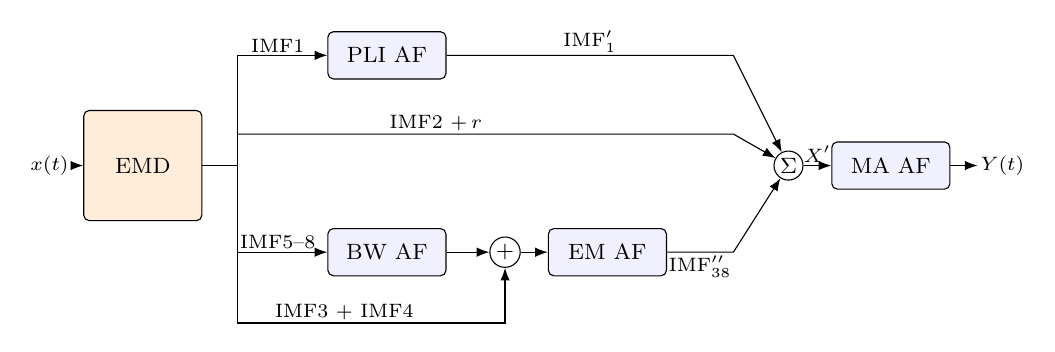
\begin{tikzpicture}
  \node[lab, anchor=east] (x) at (-0.2,0) {$x(t)$};
  \node[emd] (e) at (0.7,0) {EMD};
  \draw[->] (x) -- (e);
  \draw (e.east) -- (1.9,0);
  \draw (1.9,1.4) -- (1.9,-2.0);
  \node[blk] (pli) at (3.8,1.4) {PLI AF};
  \node[blk] (bw)  at (3.8,-1.1){BW AF};
  \node[sumn] (s2) at (5.3,-1.1) {$+$};
  \node[blk] (em)  at (6.6,-1.1){EM AF};
  \node[sumn] (S) at (8.9,0) {$\Sigma$};
  \node[blk] (ma) at (10.2,0) {MA AF};
  \node[lab, anchor=west] (y) at (11.3,0) {$Y(t)$};
  \draw[->] (1.9,1.4) -- node[lab,above,pos=0.45]{IMF1} (pli);
  \draw[->] (1.9,-1.1) -- node[lab,above,pos=0.45]{IMF5--8} (bw);
  \draw[->] (bw) -- (s2);
  \draw[->] (1.9,-2.0) -- node[lab,above,pos=0.4]{IMF3 + IMF4} (5.3,-2.0) -- (s2);
  \draw[->] (s2) -- (em);
  \draw[->] (1.9,0.4) -- node[lab,above,pos=0.4]{IMF2 $+\,r$} (8.2,0.4) -- (S);
  \draw[->] (pli.east) -- node[lab,above]{IMF$_1'$} (8.2,1.4) -- (S);
  \draw[->] (em.east) -- node[lab,below]{IMF$_{38}''$} (8.2,-1.1) -- (S);
  \draw[->] (S) -- node[lab,above]{$X'$} (ma);
  \draw[->] (ma) -- (y);
\end{tikzpicture}}
\caption{SEAF, Eq.~(\ref{eq:seaf})}
\end{subfigure}
\caption{The denoising structures as implemented, redrawn after Figs.~1, 4 and 5 of~\cite{dai} with the residue
  $r$ shown explicitly. ``AF'' is an adaptive noise canceller (a) driven by the reference of the named noise. PDAF
  is structure (a) applied to $x(t)$ with the sum of all references.}
\label{fig:struct}
\end{figure}

\subsection{Evaluation metrics}
With clean signal $x_c$, noisy signal $x_n$ and denoised signal $x_d$ (Eqs.~(4)--(6) of~\cite{dai}):
\begin{equation}
  \mathrm{SNR}=10\log_{10}\frac{\sum|x_c|^2}{\sum|x_d-x_c|^2},\quad
  \mathrm{RMSE}=\sqrt{\tfrac{1}{N}\textstyle\sum(x_d-x_c)^2},\quad
  \snrimp=10\log_{10}\frac{\sum|x_n-x_c|^2}{\sum|x_d-x_c|^2}.
\end{equation}

%======================================================================== 4
\section{Implementation Details}

\subsection{Software pipeline}
Everything was written in Python (NumPy, SciPy, \texttt{wfdb}, Numba, Matplotlib). The full codebase, with the
scripts, notebooks and all result files, is available at \url{https://github.com/LuchithaP/EMD_for_ECG}. The
project has five scripts that run in order:
\begin{enumerate}
  \item \textbf{IMF selection:} the per-noise IMF study.
  \item \textbf{Filter tuning:} the grid search of the filter settings.
  \item \textbf{BW + PLI experiments:} Figs.~6--8 of the paper.
  \item \textbf{Four-noise experiments:} Figs.~9--11 of the paper.
  \item \textbf{Comparison:} an automatic check of every claim of the paper against our numbers.
\end{enumerate}
The modules are organised as follows:
\begin{itemize}
  \item \texttt{data.py} builds the noisy cases.
  \item \texttt{emd.py} implements EMD with MATLAB \texttt{emd()} defaults: cubic-spline envelopes, sifting stopped
        at a relative tolerance of 0.2 or after 100 sifts, and 8 IMFs plus the residue.
  \item \texttt{filters.py} implements LMS, NLMS and RLS. The sample loops are compiled with Numba.
  \item \texttt{methods.py} implements Eq.~(1), PEAF, SEAF, SDAF and PDAF.
  \item \texttt{metrics.py} implements Eqs.~(4)--(6).
\end{itemize}
Every setting is kept in one configuration file. Each setting is marked either \textsc{[paper]} (taken from the paper)
or \textsc{[ours]} (our choice where the paper gives none).

\subsection{Construction of the noisy signals}
\begin{itemize}
  \item \textbf{Segment:} each record has 650{,}000 samples; we used the first 65{,}000 (about 3\,min, 10\,\%) to
        keep the computation manageable (Sec.~\ref{sec:challenges}).
  \item \textbf{ECG scaling:} each ECG was made zero-mean and scaled to $\max|x|=1$. In the paper's Figs.~6 and 9 the
        clean ECG sits at a baseline of about 0 with R peaks of about 1, and the RMSE/SNR pairs of Fig.~7 imply a
        clean-ECG RMS of about 0.16. Our ECGs have an RMS of 0.11--0.25.
  \item \textbf{References:} the paper states that the added noises were \emph{``shifted and passed through different
        filters to get noises that are not equal but correlated to the adaptive filters' reference noises''}. We
        therefore used each NSTDB record (in mV, mean removed) as the reference $n_k$ and added a delayed, FIR-filtered
        copy to the ECG:
        \begin{equation}
          x(t)=s(t)+g\sum_k (h_k * n_k)(t-D_k).
        \end{equation}
        The paths were BW: $D=5$, $h=[0.5,0.3,0.2]$; EM: $D=3$, $h=[0.6,0.3,0.1]$; MA: $D=2$, $h=[0.7,0.2,0.1]$. The
        added PLI was phase-shifted by $45^\circ$ against its reference.
  \item \textbf{Noise mix:} the NSTDB noises keep their natural power ratio (EM 46.6\,\%, BW 24.7\,\%, MA 3.9\,\%),
        and the PLI was given the power of BW. A single gain $g$ sets the exact $\snrin$. The references were
        \emph{not} rescaled with $\snrin$, as for a real reference electrode, so a given step size behaves the same at
        every $\snrin$.
\end{itemize}

\subsection{Filter parameter tuning}
\label{sec:tuning}
The paper only states that \emph{``default parameters in MATLAB''} were used. The step size and filter length
together decide whether an LMS canceller converges at all, because the stability bound depends on the reference power
$P_u$. A naive single setting (for example 32 taps with $\mu=0.1$) diverged for the BW filter under our reference
scaling (blank cells in Fig.~\ref{fig:tuning}). We therefore tuned every filter of every method separately:
\begin{itemize}
  \item \textbf{Grid:} LMS $\mu\in\{10^{-5},3{\cdot}10^{-5},\dots,3\}$ (12 values); NLMS $\mu\in[10^{-3},1]$
        (7 values); RLS $\lambda\in\{0.99,\dots,1\}$ (6 values) with $\mathbf{P}(0)=1000\,\mathbf{I}$; filter length
        $L\in\{1,2,4,\dots,64\}$.
  \item \textbf{Search:} coordinate descent. The search starts with all filters off. Each filter in turn takes the grid
        setting that maximises the mean $\snrimp$ while the other filters stay fixed, and two full passes are made.
        Any setting that diverged in any case was rejected.
  \item \textbf{Held-out data:} the tuning used records 101, 112, 117, 201 and 220, which appear in no figure, with
        $\snrin\in\{-5,0,5,10\}$\,dB and a different noise segment (starting at sample 325{,}000). The test
        figures therefore do not reuse the tuning data.
  \item \textbf{One setting per filter:} a single setting per filter is used for all $\snrin$, as the paper does.
\end{itemize}
Table~\ref{tab:params} lists the tuned settings. Fig.~\ref{fig:tuning} shows two of the tuning surfaces.

\begin{table}[!htbp]
\centering\small
\caption{Tuned filter settings: $(\mu, L)$ for LMS/NLMS and $(\lambda, L)$ for RLS.}
\label{tab:params}
\begin{tabular}{lcccc}
\toprule
Method & PLI filter & BW filter & EM filter & MA filter\\
\midrule
EMD+LMS  & $10^{-2}$, 16 & $3{\cdot}10^{-4}$, 8 & -- & -- \\
EMD+NLMS & $3{\cdot}10^{-2}$, 16 & $10^{-3}$, 64 & -- & -- \\
EMD+RLS  & $\lambda{=}1$, 4 & $\lambda{=}1$, 8 & -- & -- \\
PEAF     & $3{\cdot}10^{-2}$, 4 & $3{\cdot}10^{-5}$, 32 & $10^{-4}$, 8 & $3{\cdot}10^{-3}$, 4 \\
SEAF     & $3{\cdot}10^{-2}$, 4 & $10^{-4}$, 8 & $10^{-4}$, 8 & $3{\cdot}10^{-3}$, 4 \\
SDAF     & $3{\cdot}10^{-3}$, 16 & $10^{-4}$, 8 & $10^{-4}$, 8 & $3{\cdot}10^{-3}$, 4 \\
PDAF     & \multicolumn{4}{c}{one filter, summed references: $3{\cdot}10^{-4}$, 8}\\
\bottomrule
\end{tabular}
\end{table}

The tuning gave three insights:
\begin{enumerate}
  \item The optimal step sizes span \textbf{three orders of magnitude} ($3{\cdot}10^{-5}$ to $3{\cdot}10^{-2}$). The
        reason is that the input of each canceller (IMF1, the IMF5--8 sum, or the full signal) and each reference have
        very different powers.
  \item The optimal settings depend on the structure. The BW filter of PEAF prefers a much smaller $\mu$ and a longer
        filter than the BW filter of SEAF, because in PEAF it works on IMFs that still contain the EM noise.
  \item A single fixed setting is a compromise across $\snrin$. In a preliminary single-filter sweep, the best fixed
        $(\mu,L)$ lost 0.9--2.1\,dB against the best setting chosen separately for each $\snrin$.
\end{enumerate}
These observations motivate the variable step-size proposal in Sec.~\ref{sec:vss}.

\begin{figure}[!htbp]
\centering
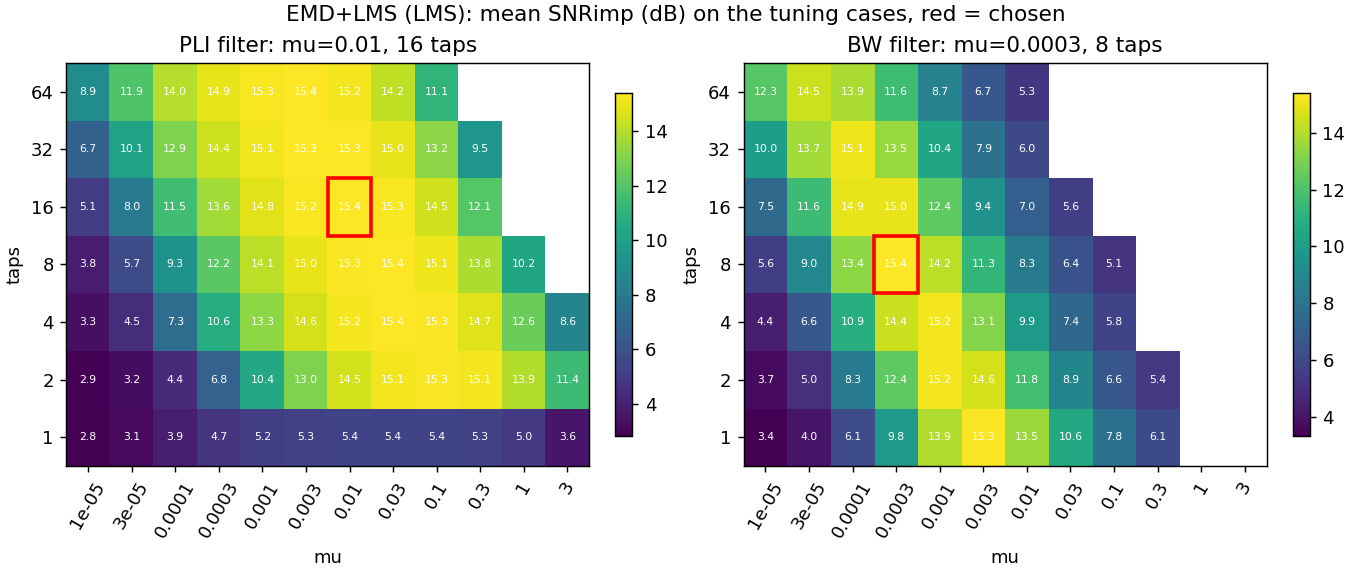
\includegraphics[width=0.329\textwidth]{filter_tuning_mean_snr_imp_emd_lms.png}\hfill
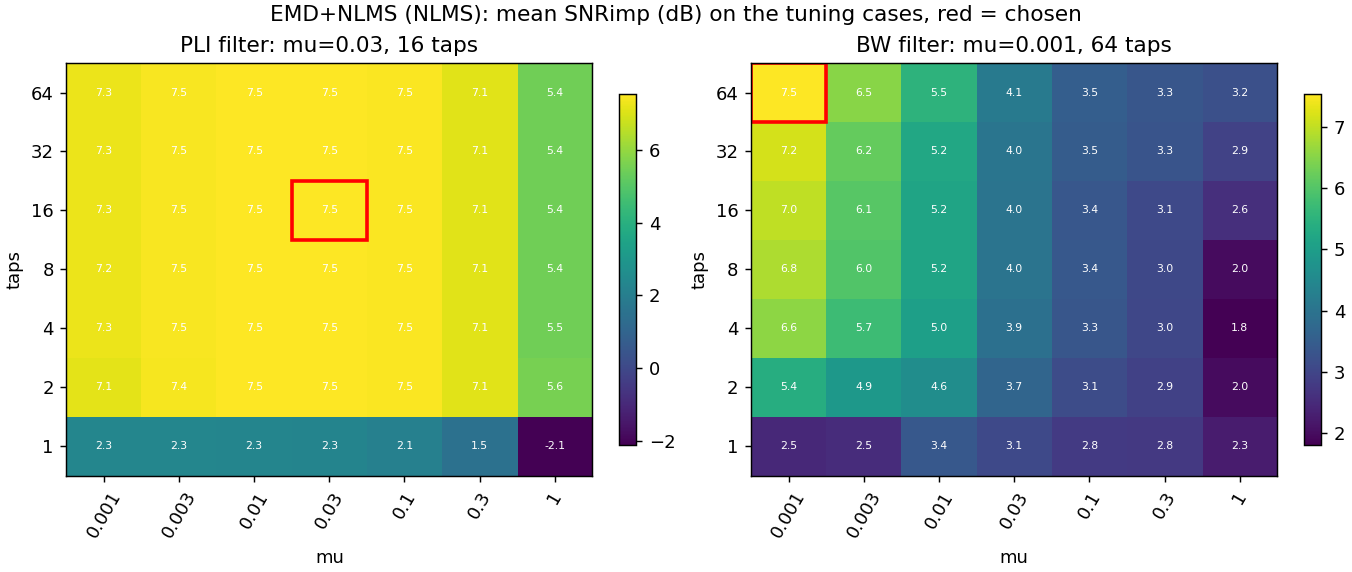
\includegraphics[width=0.329\textwidth]{filter_tuning_mean_snr_imp_emd_nlms.png}\hfill
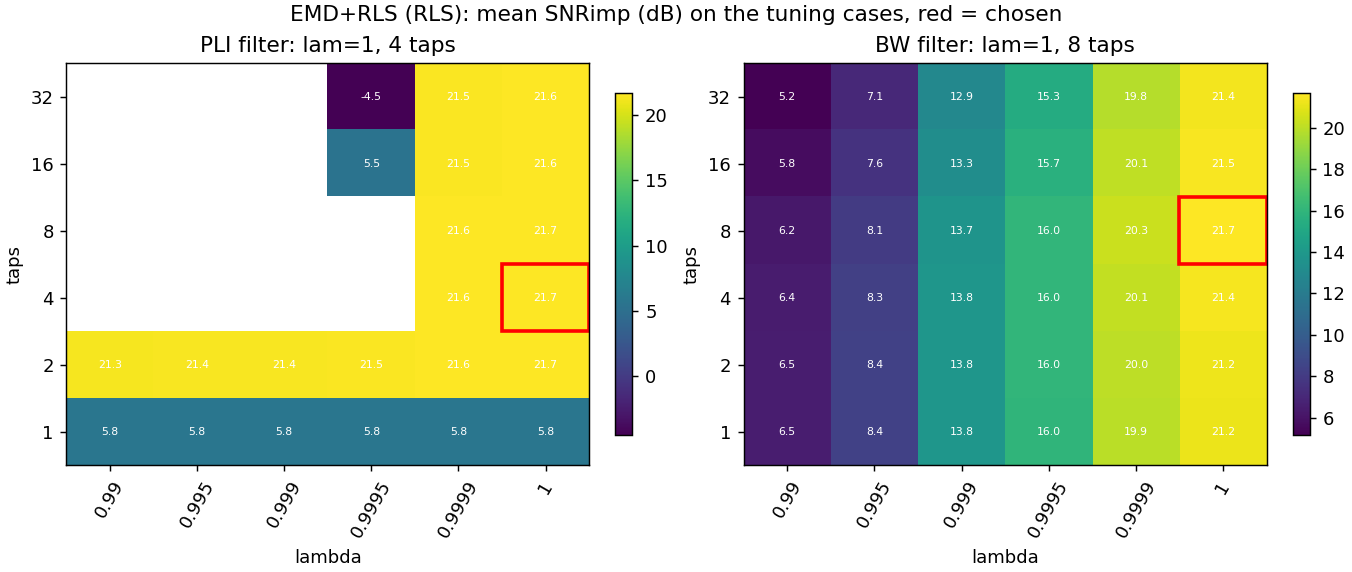
\includegraphics[width=0.329\textwidth]{filter_tuning_mean_snr_imp_emd_rls.png}\\[2mm]
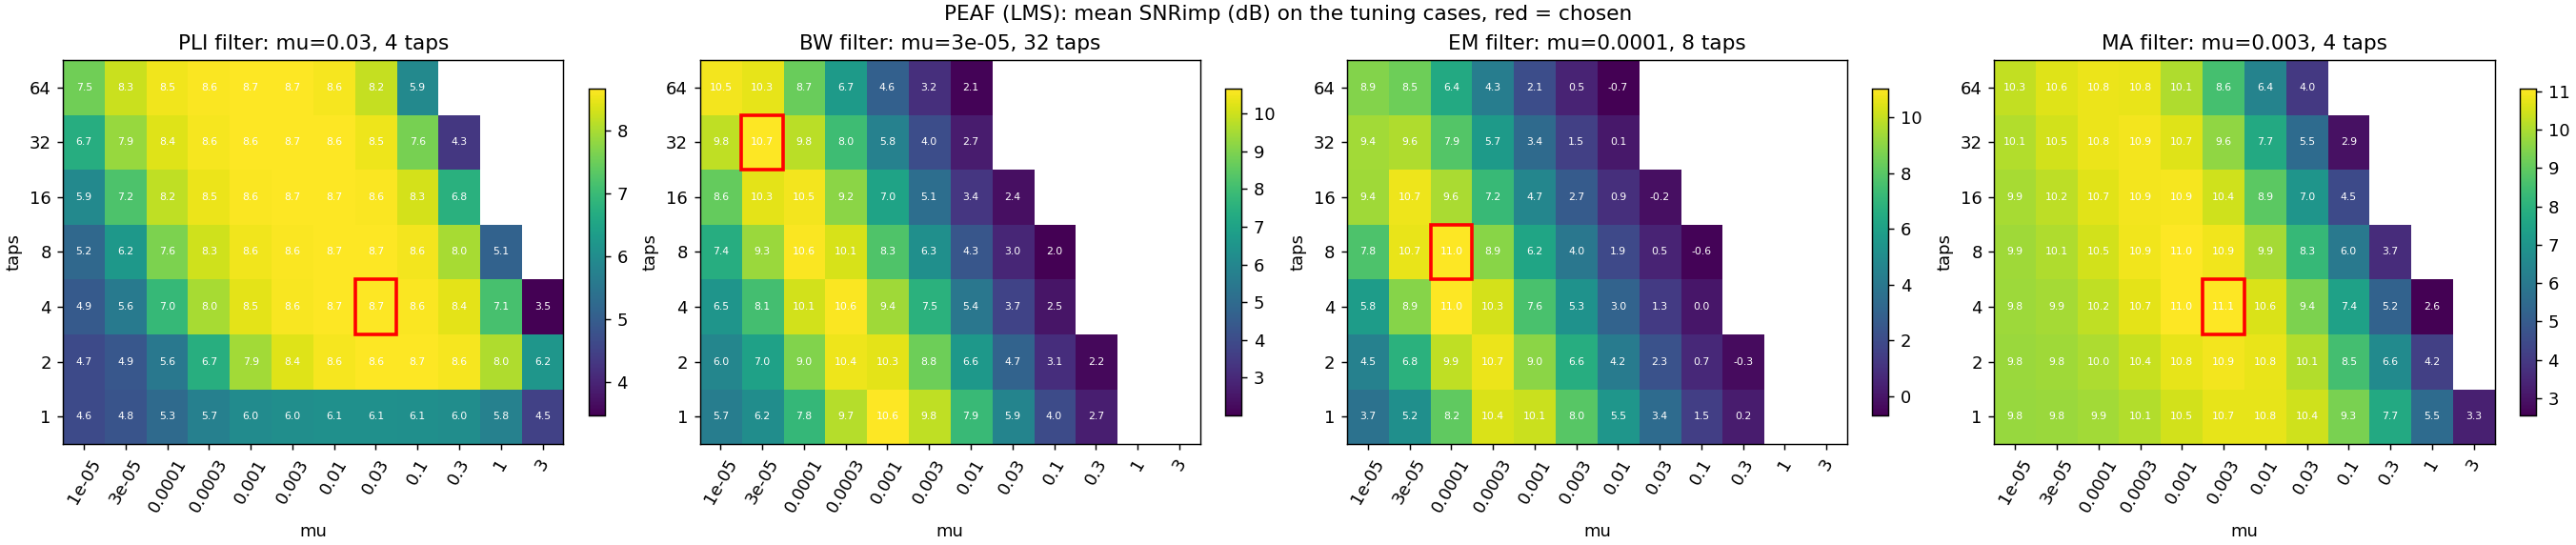
\includegraphics[width=\textwidth]{filter_tuning_mean_snr_imp_peaf.png}
\caption{Tuning surfaces: mean $\snrimp$ on the held-out cases, with the chosen setting boxed in red. Top: EMD+LMS,
  EMD+NLMS ($\mu$, $L$) and EMD+RLS ($\lambda$, $L$) for BW + PLI. Bottom: the four LMS filters of PEAF. Blank cells
  are settings that diverged.}
\label{fig:tuning}
\end{figure}

\subsection{Challenges faced}
\label{sec:challenges}
\begin{itemize}
  \item \textbf{Computational cost.} Each MIT-BIH and NSTDB record is 650{,}000 samples long (30\,min at 360\,Hz).
        Running EMD and thousands of tuning runs on full records was not feasible, so we used 65{,}000 samples (10\,\%)
        of each record. Even at this length, EMD of one signal takes seconds and the grid search needs thousands of
        filter runs, so the pipeline was still computationally expensive. To make it practical we cached every EMD
        result by a hash of its input, compiled the filters with Numba, cached unchanged filter outputs during
        coordinate descent, and parallelised over 8 cores. The full pipeline then runs in about 20 minutes.
  \item \textbf{Divergence.} Many grid points make LMS unstable. A divergence detector (non-finite output, or output
        power far above input power) rejects these settings.
  \item \textbf{Ambiguities.} The ambiguities are listed in Sec.~\ref{sec:limits}. Where the paper allows two readings
        (e.g.\ the $\snrin$ of Fig.~10) we report both.
\end{itemize}

%======================================================================== 5
\section{Implementation Results and Comparison with the Paper}

\subsection{EMD of a noisy ECG and IMF selection}
Fig.~\ref{fig:emd} shows the EMD of an ECG corrupted by all four noises. The 60\,Hz line is isolated in IMF1. The QRS
energy is spread over IMF1--IMF4, and the slow drift sits in IMF6--IMF8. Fig.~\ref{fig:imfsel} shows the results of
the IMF selection study.

\begin{figure}[!htbp]
\centering
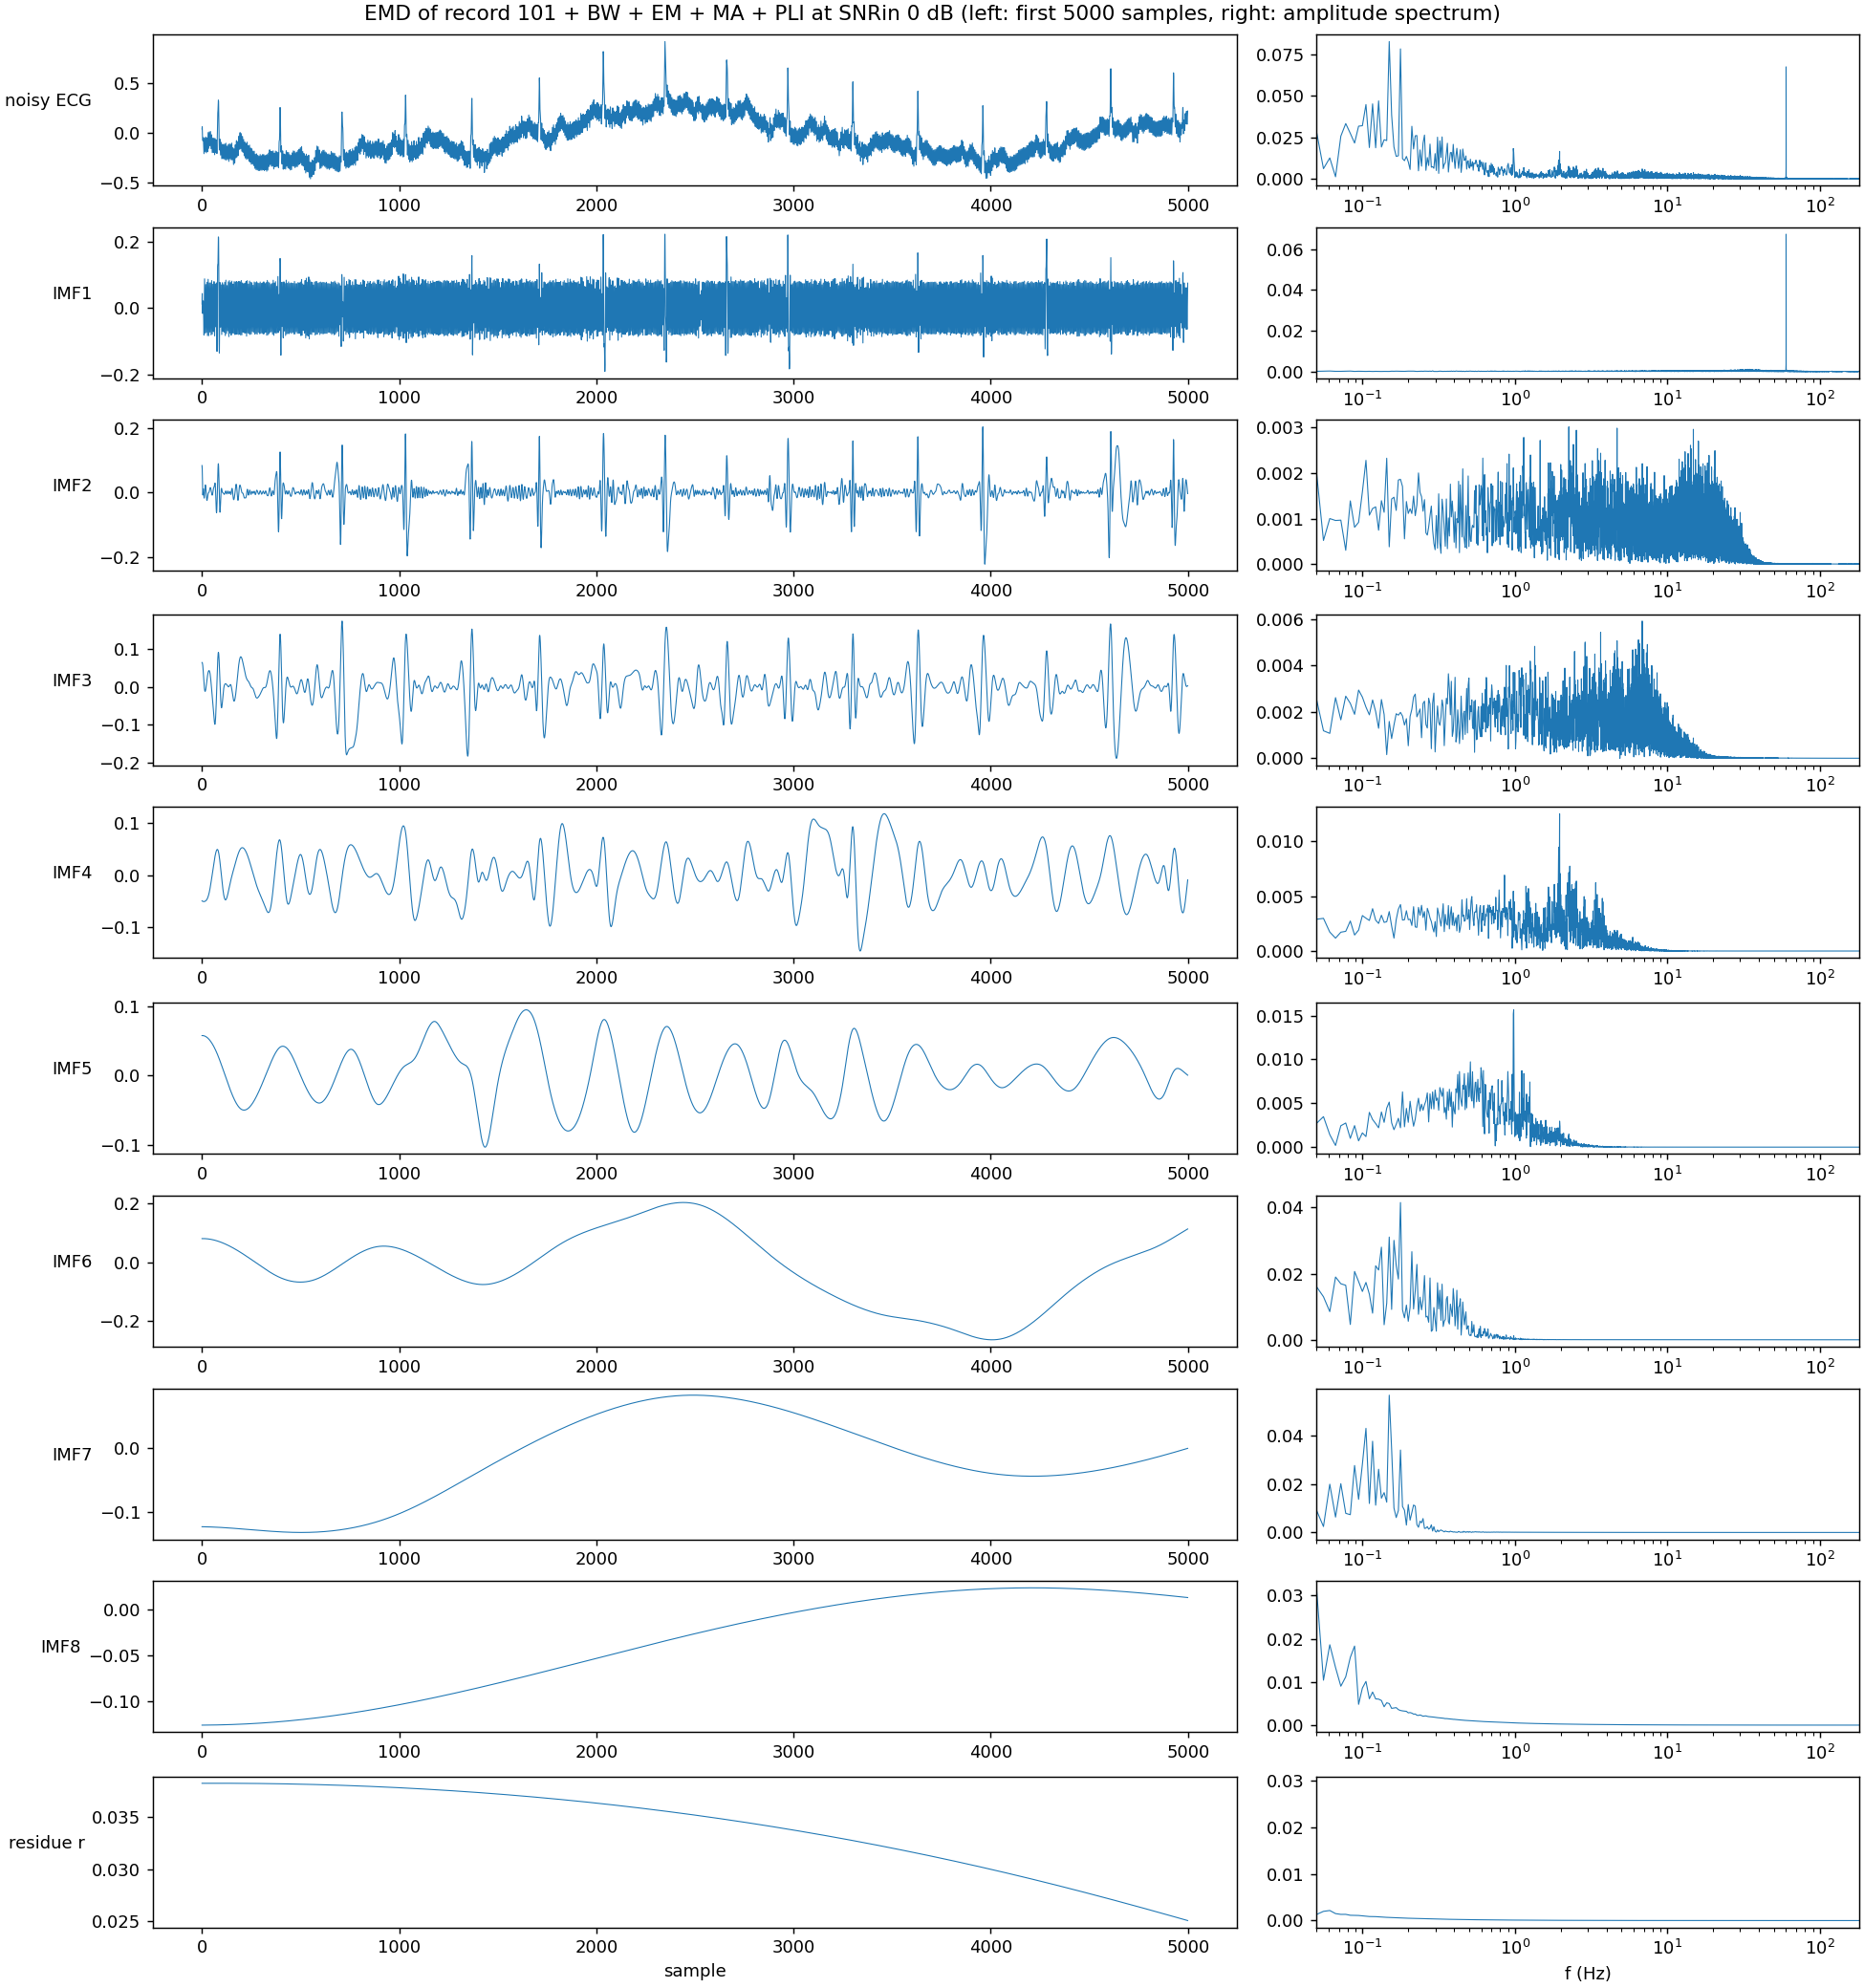
\includegraphics[width=0.56\textwidth]{emd_imfs_and_spectra_of_noisy_ecg.png}
\caption{EMD of record 101 + BW + EM + MA + PLI at $\snrin=0$\,dB. Left: first 5000 samples of each IMF. Right:
  amplitude spectra on a log-frequency axis.}
\label{fig:emd}
\end{figure}

\begin{figure}[!htbp]
\centering
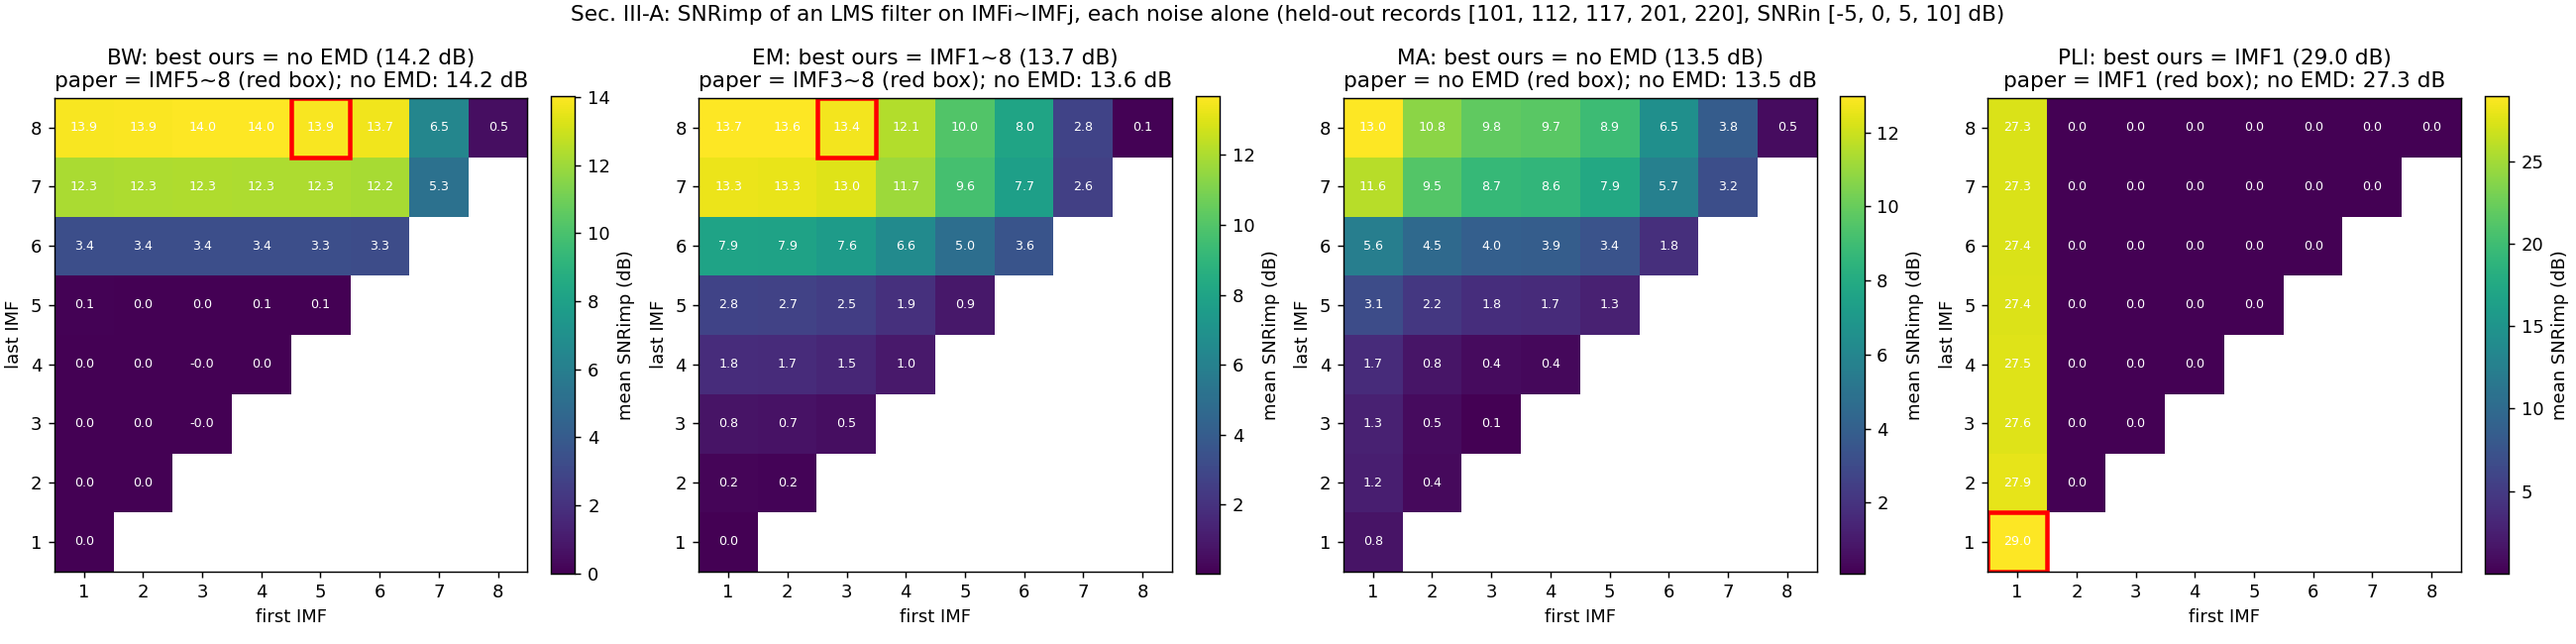
\includegraphics[width=\textwidth]{imf_selection_snr_imp_per_imf_range.png}
\caption{IMF selection (Sec.~III-A of~\cite{dai}): mean $\snrimp$ of an LMS canceller on $\imf{i}\!\sim\!\imf{j}$
  for each noise alone (held-out cases). The paper's choice is boxed in red.}
\label{fig:imfsel}
\end{figure}

\begin{table}[!htbp]
\centering\small
\caption{IMF selection: best range found by us against the paper's choice (mean $\snrimp$, dB).}
\label{tab:imf}
\begin{tabular}{lccccl}
\toprule
Noise & Our best & $\snrimp$ & Paper's choice & $\snrimp$ & No EMD\\
\midrule
PLI & IMF1   & 28.98 & IMF1   & 28.98 & 27.31\\
BW  & no EMD & 14.22 & IMF5--8 & 13.88 & 14.22\\
EM  & IMF1--8 & 13.69 & IMF3--8 & 13.45 & 13.57\\
MA  & no EMD & 13.47 & no EMD & 13.47 & 13.47\\
\bottomrule
\end{tabular}
\end{table}

\begin{itemize}
  \item \textbf{PLI and MA:} the paper's choice is reproduced exactly.
  \item \textbf{BW and EM:} the paper's ranges are within 0.35\,dB of the best range. This is about the spread between
        neighbouring grid settings, so the paper's ranges are near-optimal and we kept them.
  \item \textbf{BW:} every range that ends at IMF8 gives about 14\,dB, while ranges that end at IMF6 or below give
        $\le3.4$\,dB.
\end{itemize}

\subsection{BW + PLI denoising}
Fig.~\ref{fig:bwpli_ex} shows an example of BW + PLI denoising. The 60\,Hz line and the drift are removed, and the
waveform morphology is preserved. As in the paper, the output is poorer during the first few seconds while the filter
converges.

\begin{figure}[!htbp]
\centering
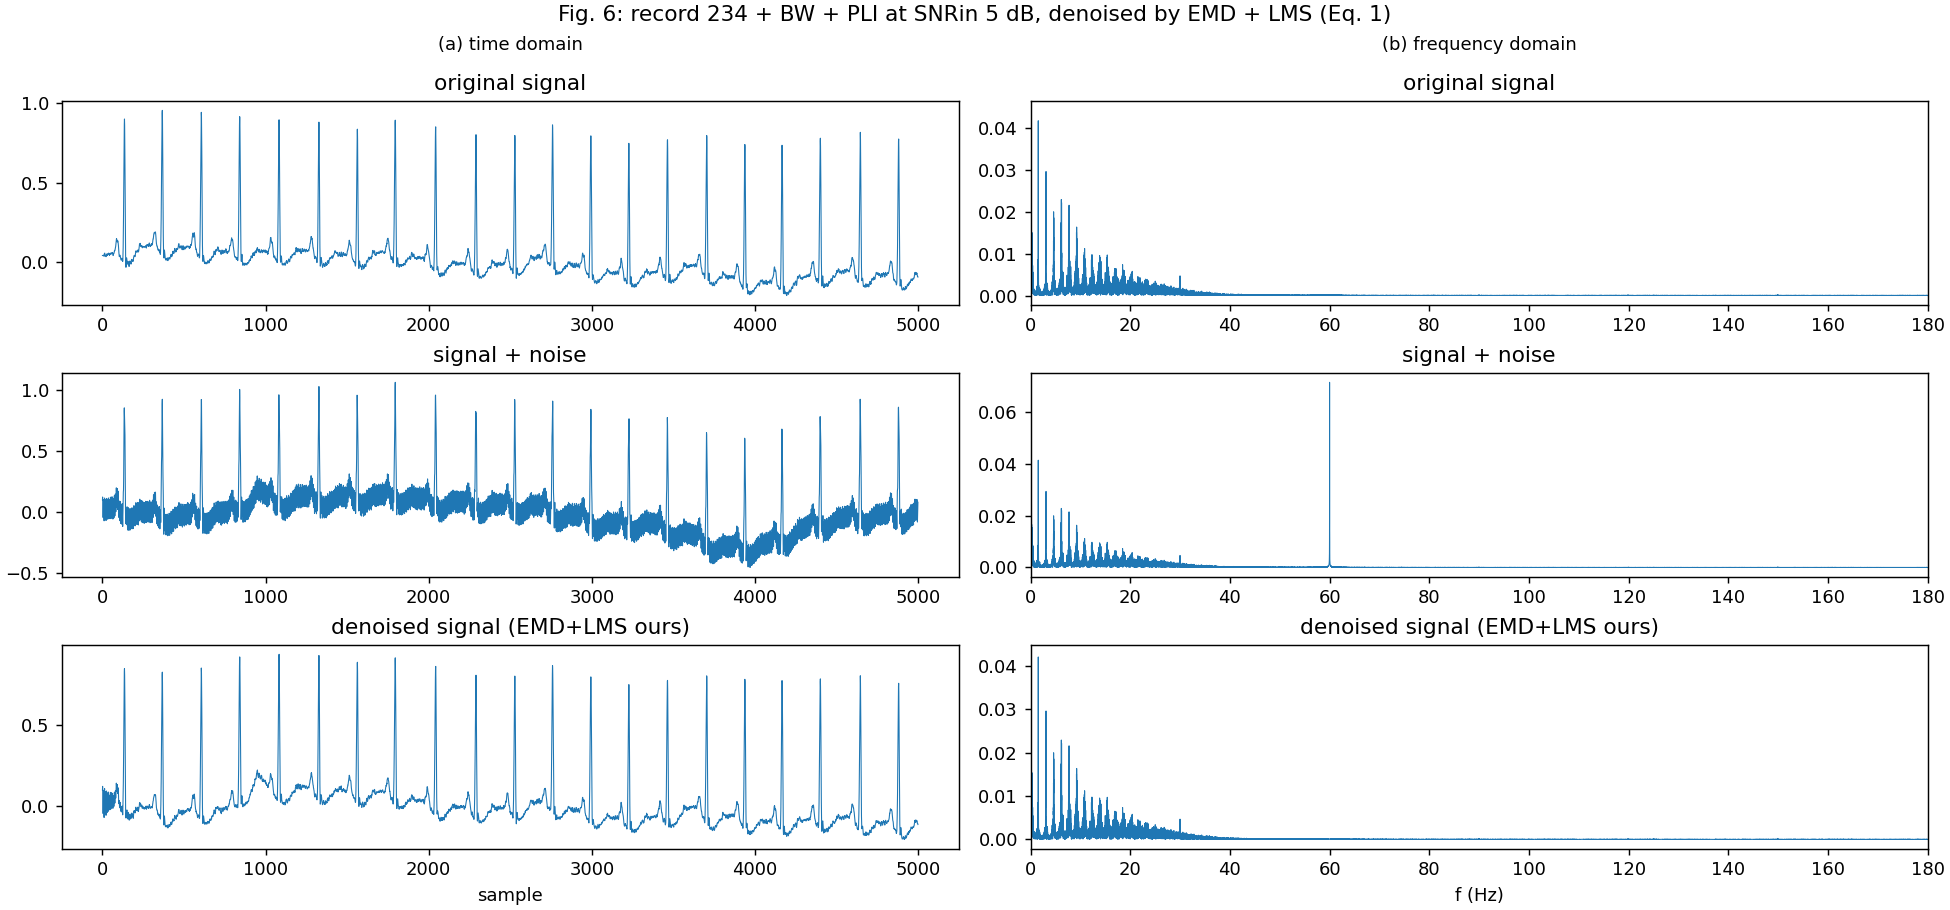
\includegraphics[width=0.85\textwidth]{fig6_bw_pli_example_emd_lms_record234_snr5dB.png}
\caption{Counterpart of Fig.~6 of~\cite{dai}: record 234 + BW + PLI at $\snrin=5$\,dB, denoised by EMD+LMS.}
\label{fig:bwpli_ex}
\end{figure}

\begin{figure}[!htbp]
\centering
\begin{subfigure}{0.495\textwidth}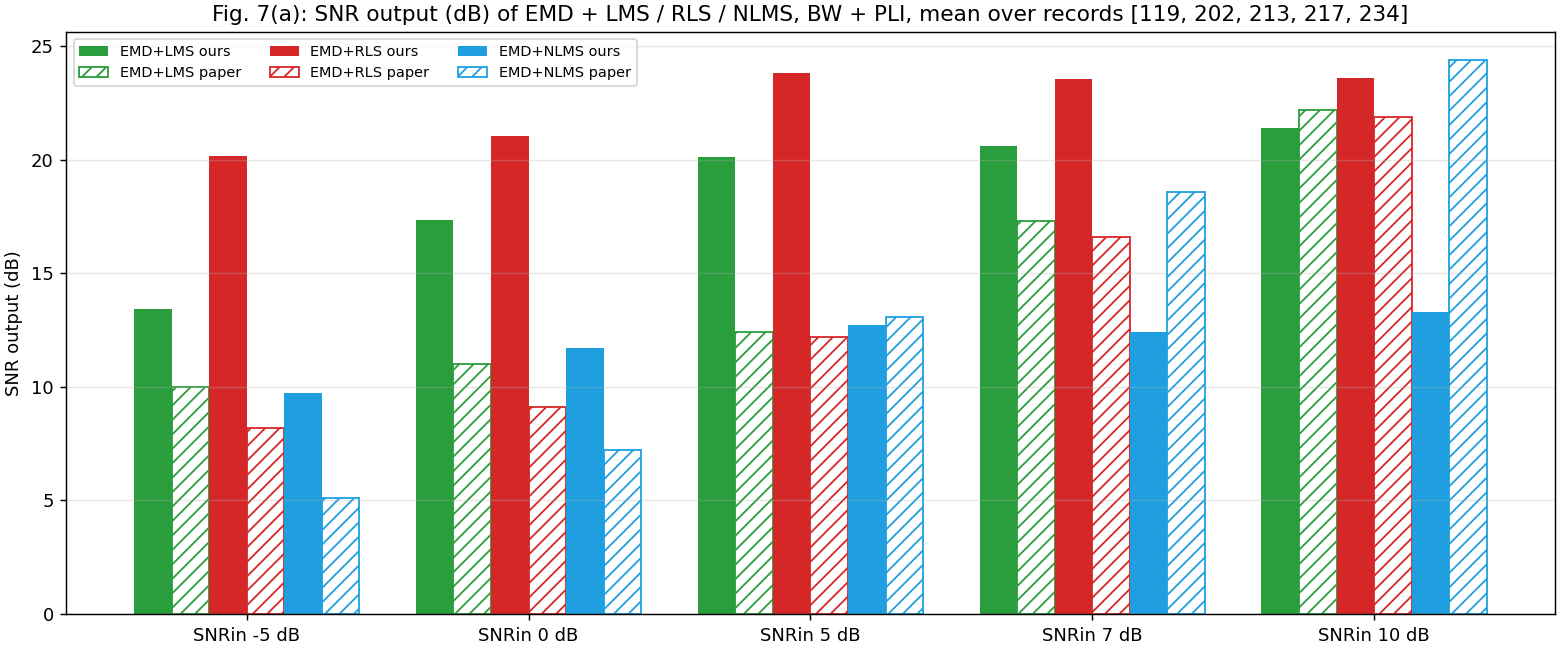
\includegraphics[width=\textwidth]{fig7a_snr_out_lms_rls_nlms_vs_snr_in_bw_pli.png}\caption{$\snrout$}\end{subfigure}\hfill
\begin{subfigure}{0.495\textwidth}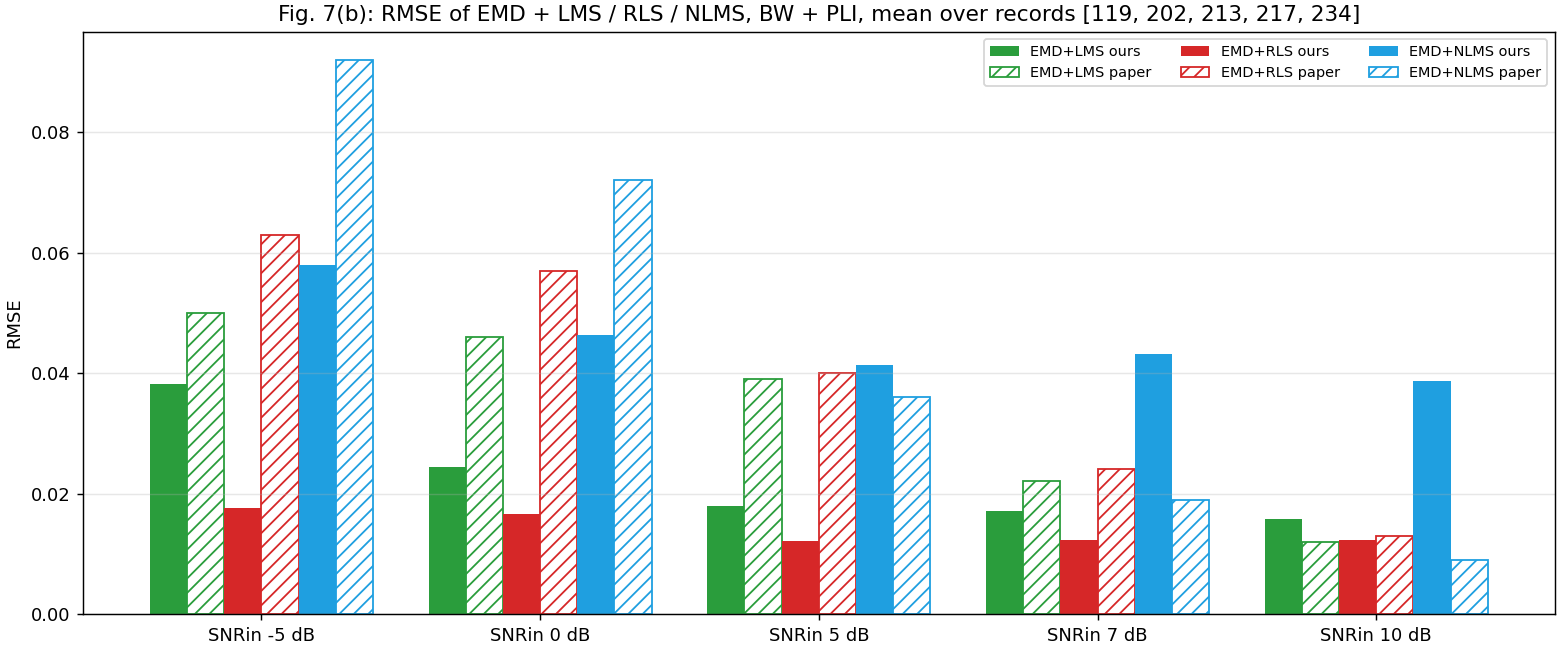
\includegraphics[width=\textwidth]{fig7b_rmse_lms_rls_nlms_vs_snr_in_bw_pli.png}\caption{RMSE}\end{subfigure}
\caption{Counterpart of Fig.~7 of~\cite{dai}. Solid bars: ours; hatched bars: values read from the paper.}
\label{fig:fig7}
\end{figure}

\begin{table}[!htbp]
\centering\small
\caption{BW + PLI: mean $\snrout$ (dB) over records 119, 202, 213, 217, 234. Each cell is \textbf{ours} (paper).}
\label{tab:fig7}
\begin{tabular}{lccccc}
\toprule
$\snrin$ (dB) & $-5$ & 0 & 5 & 7 & 10\\
\midrule
EMD+LMS  & \textbf{13.4} (10.0) & \textbf{17.3} (11.0) & \textbf{20.1} (12.4) & \textbf{20.6} (17.3) & \textbf{21.4} (22.2)\\
EMD+RLS  & \textbf{20.2} (8.2)  & \textbf{21.0} (9.1)  & \textbf{23.8} (12.2) & \textbf{23.6} (16.6) & \textbf{23.6} (21.9)\\
EMD+NLMS & \textbf{9.8} (5.1)   & \textbf{11.7} (7.2)  & \textbf{12.7} (13.1) & \textbf{12.4} (18.6) & \textbf{13.3} (24.4)\\
\bottomrule
\end{tabular}
\end{table}

\textbf{LMS, NLMS and RLS (Fig.~\ref{fig:fig7}, Table~\ref{tab:fig7}):}
\begin{itemize}
  \item Our EMD+LMS is above the paper's value up to $\snrin=7$\,dB and 0.8\,dB below it at 10\,dB.
  \item Our $\snrout$ saturates near 21--24\,dB, while the paper's keeps rising with $\snrin$.
  \item With tuned settings, RLS ($\lambda=1$) is the best canceller at every $\snrin$. The paper selects LMS.
\end{itemize}

\textbf{Fig.~8, $\snrin=10$\,dB:} our EMD+LMS gives 24.9, 19.5, 23.7, 20.3 and 18.9\,dB on records 119, 202, 213,
217 and 234. The paper reports 24.7, 22.9, 25.0, 29.2 and 23.9\,dB. Our implementation therefore exceeds the best of
the values reported for articles [21, 22, 28] of~\cite{dai} on 2 of the 5 records (Fig.~\ref{fig:fig8}).

\begin{figure}[!htbp]
\centering
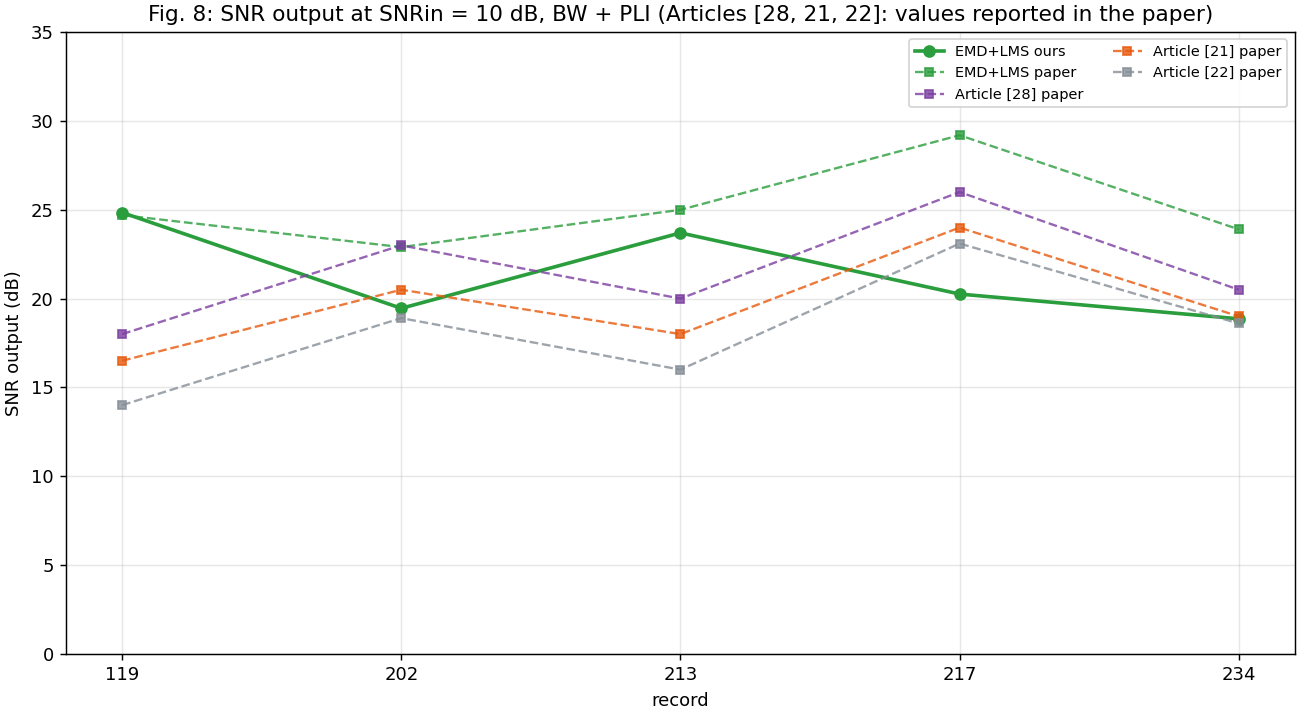
\includegraphics[width=0.6\textwidth]{fig8_snr_out_per_record_emd_lms_vs_articles_snr_in_10dB.png}
\caption{Counterpart of Fig.~8 of~\cite{dai}: EMD+LMS against the values reported for articles [21, 22, 28] of~\cite{dai}
  at $\snrin=10$\,dB.}
\label{fig:fig8}
\end{figure}

\subsection{BW + PLI + EM + MA denoising}
Fig.~\ref{fig:fig9} shows the PEAF output on record 100. The 60\,Hz peak and the drift are removed, and the waveform
is close to the original.

\begin{figure}[!htbp]
\centering
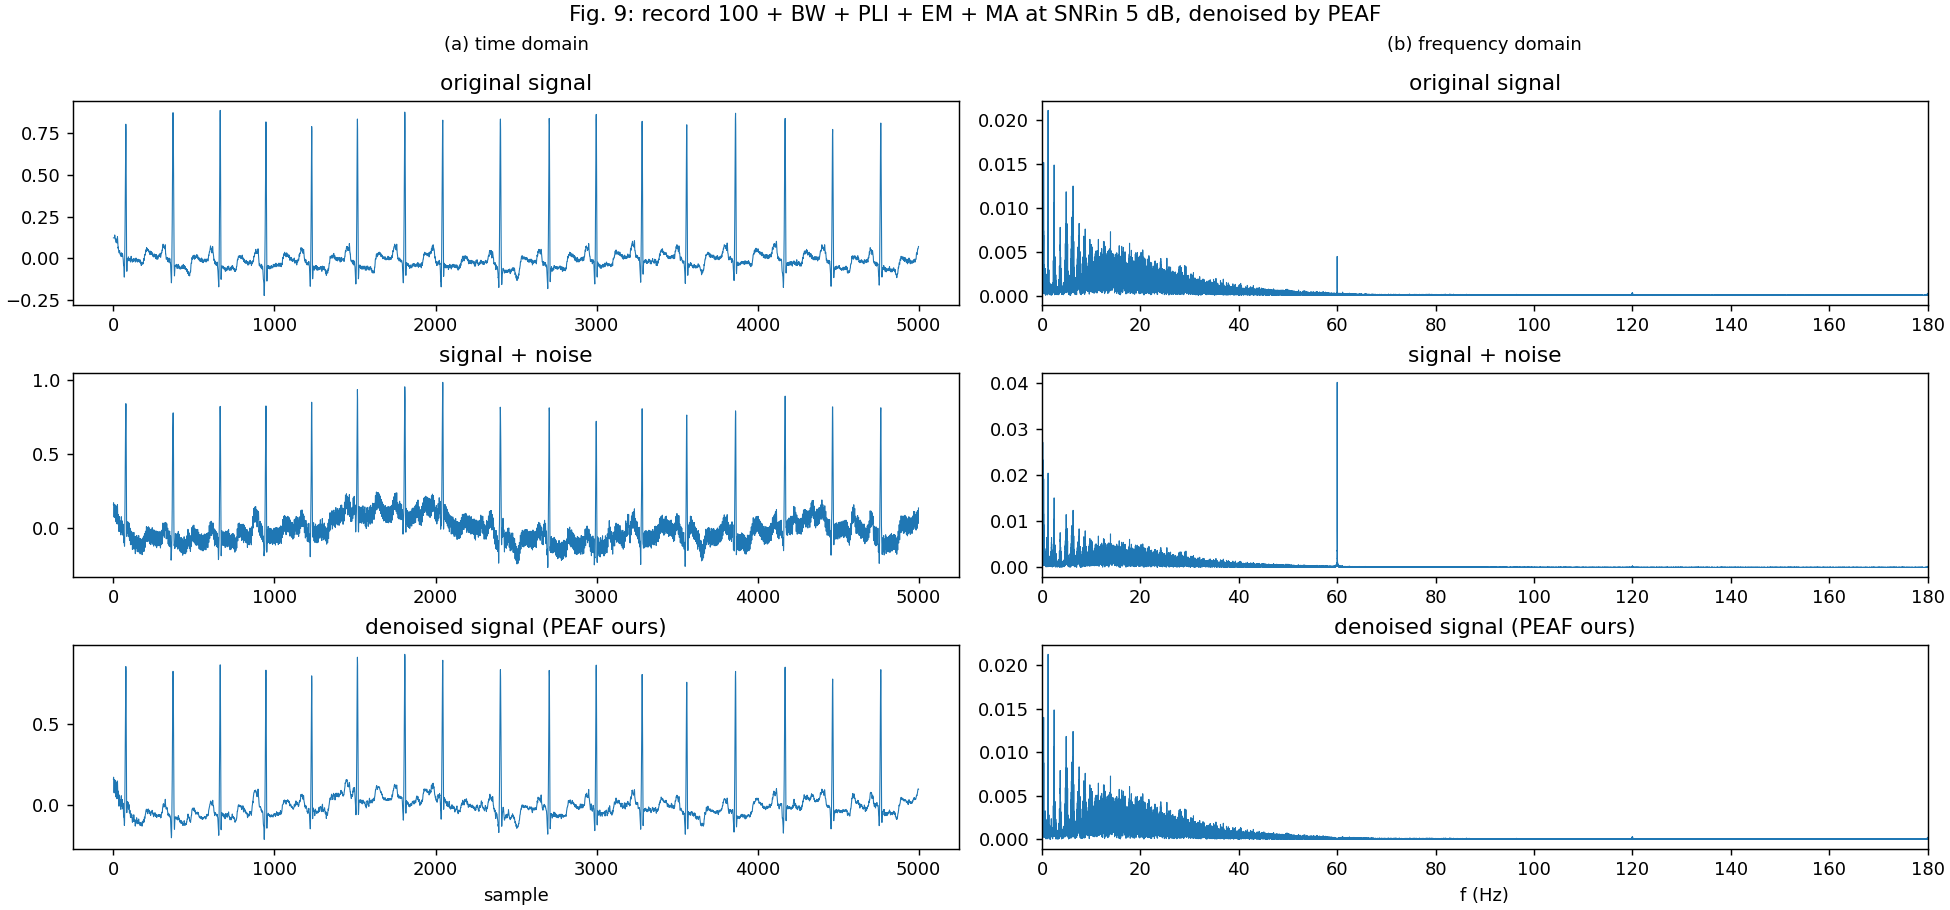
\includegraphics[width=0.85\textwidth]{fig9_four_noise_example_peaf_record100_snr5dB.png}
\caption{Counterpart of Fig.~9 of~\cite{dai}: record 100 with all four noises at $\snrin=5$\,dB, denoised by PEAF.}
\label{fig:fig9}
\end{figure}

\begin{figure}[!htbp]
\centering
\begin{subfigure}{0.495\textwidth}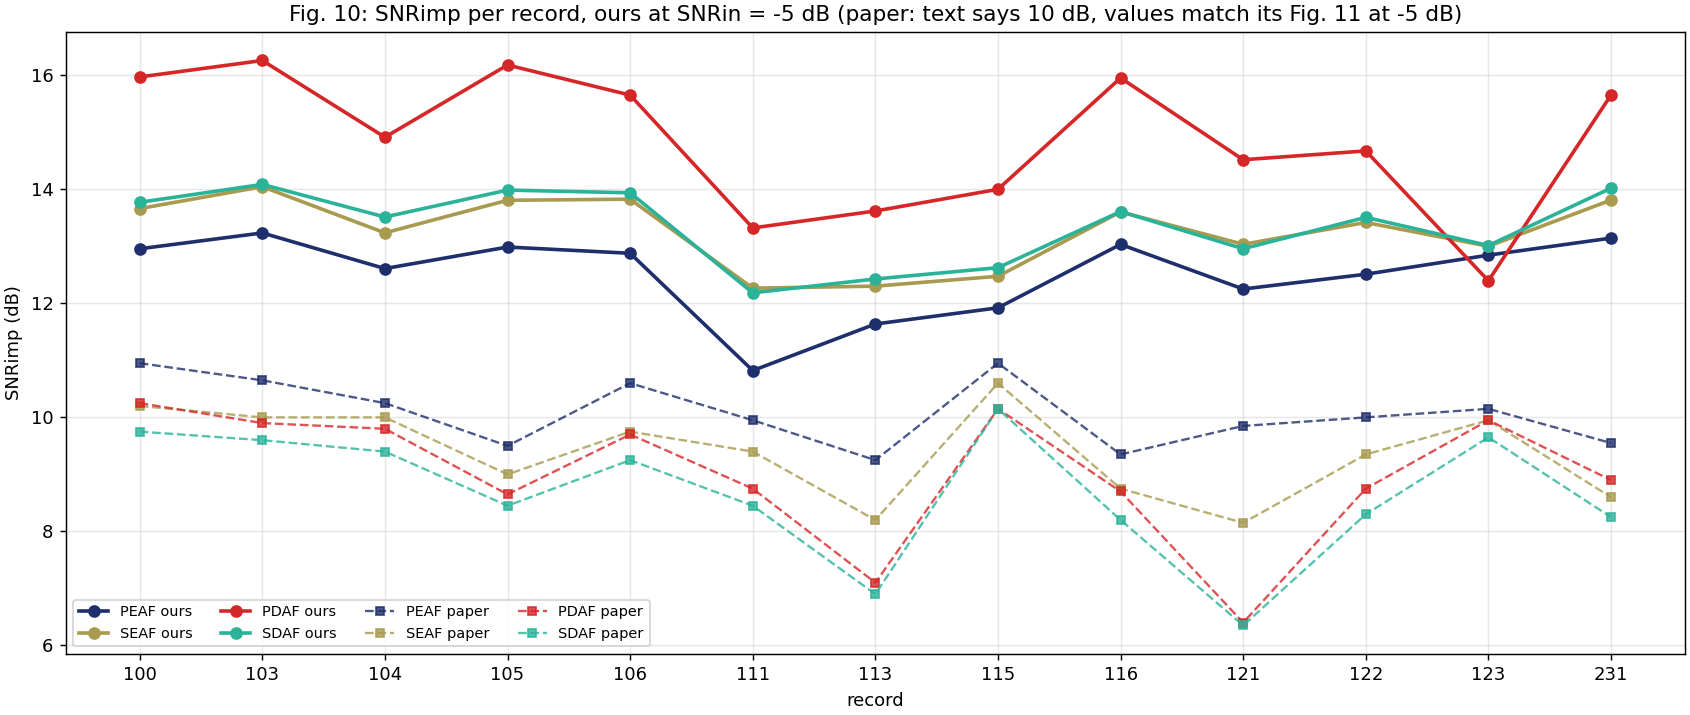
\includegraphics[width=\textwidth]{fig10_snr_imp_per_record_four_methods_snr_in_minus5dB.png}\caption{$\snrin=-5$\,dB}\end{subfigure}\hfill
\begin{subfigure}{0.495\textwidth}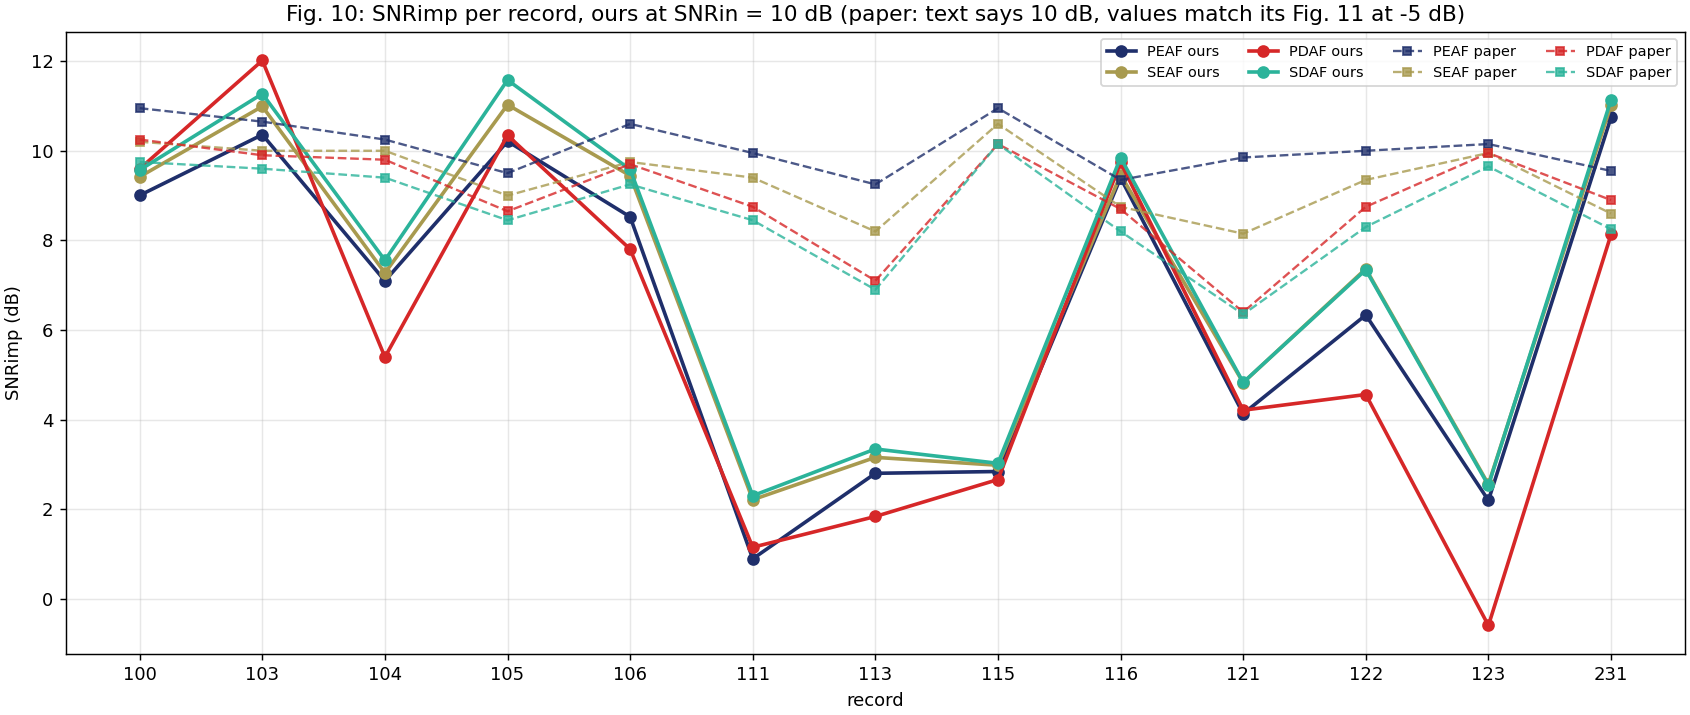
\includegraphics[width=\textwidth]{fig10_snr_imp_per_record_four_methods_snr_in_10dB.png}\caption{$\snrin=10$\,dB}\end{subfigure}
\caption{Counterpart of Fig.~10 of~\cite{dai}: $\snrimp$ per record. The paper's values are dashed.}
\label{fig:fig10}
\end{figure}

\begin{figure}[!htbp]
\centering
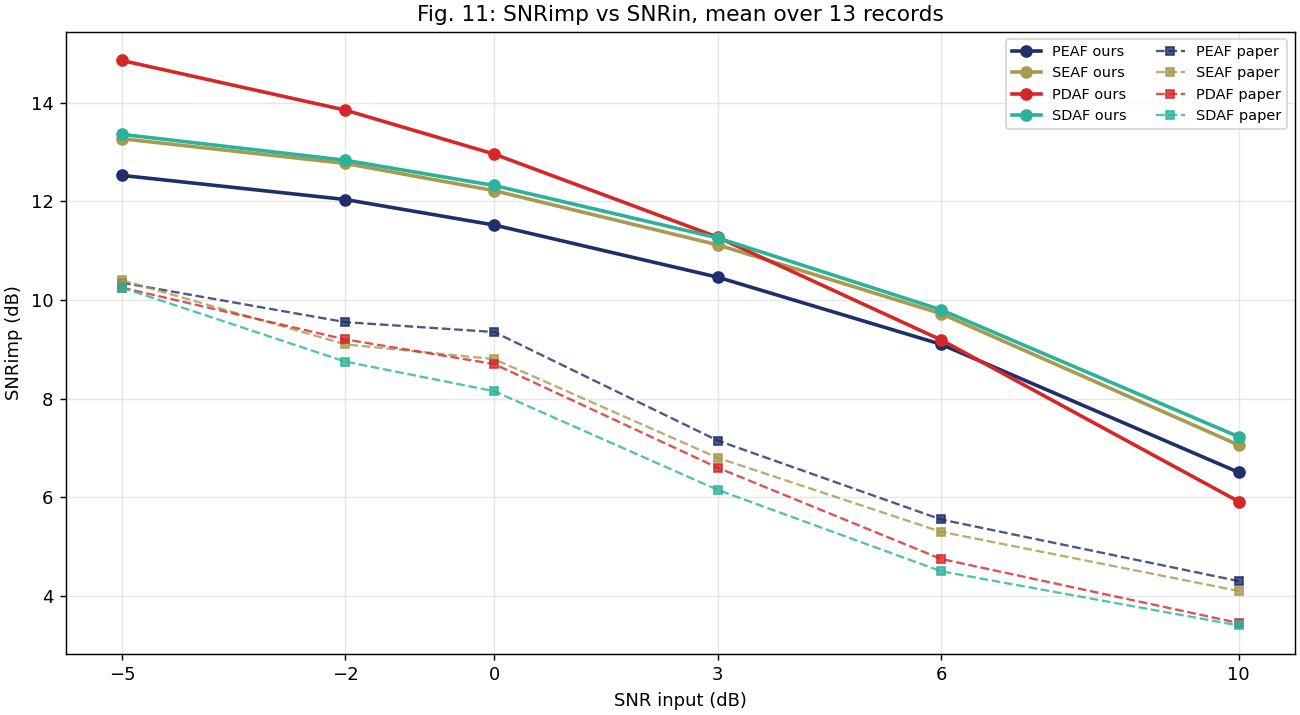
\includegraphics[width=0.62\textwidth]{fig11_snr_imp_vs_snr_in_four_methods.png}
\caption{Counterpart of Fig.~11 of~\cite{dai}: mean $\snrimp$ over the 13 records. Solid lines: ours; dashed lines:
  paper.}
\label{fig:fig11}
\end{figure}

\begin{table}[!htbp]
\centering\small
\caption{Four noises: mean $\snrimp$ (dB) over 13 records. Each cell is \textbf{ours} (paper); our best method at
  each $\snrin$ is underlined.}
\label{tab:fig11}
\begin{tabular}{lcccccc}
\toprule
$\snrin$ (dB) & $-5$ & $-2$ & 0 & 3 & 6 & 10\\
\midrule
PEAF & \textbf{12.5} (10.4) & \textbf{12.0} (9.6) & \textbf{11.5} (9.4) & \textbf{10.5} (7.2) & \textbf{9.1} (5.6) & \textbf{6.5} (4.3)\\
SEAF & \textbf{13.3} (10.4) & \textbf{12.8} (9.1) & \textbf{12.2} (8.8) & \textbf{11.1} (6.8) & \textbf{9.7} (5.3) & \textbf{7.1} (4.1)\\
PDAF & \underline{\textbf{14.9}} (10.3) & \underline{\textbf{13.9}} (9.2) & \underline{\textbf{13.0}} (8.7) & \underline{\textbf{11.3}} (6.6) & \textbf{9.2} (4.8) & \textbf{5.9} (3.5)\\
SDAF & \textbf{13.4} (10.3) & \textbf{12.8} (8.8) & \textbf{12.3} (8.2) & \textbf{11.3} (6.2) & \underline{\textbf{9.8}} (4.5) & \underline{\textbf{7.2}} (3.4)\\
\bottomrule
\end{tabular}
\end{table}

\textbf{The four methods (Figs.~\ref{fig:fig10}--\ref{fig:fig11}, Table~\ref{tab:fig11}):}
\begin{itemize}
  \item As in the paper, $\snrimp$ decreases as $\snrin$ increases for every method.
  \item Our values are 2--5\,dB higher than the paper's.
  \item The ranking differs. PDAF is best from $-5$ to 3\,dB and SDAF at 6 and 10\,dB. SEAF beats PEAF at every
        $\snrin$, by 0.5--0.8\,dB.
  \item PEAF is the lowest of the four methods at 5 of the 6 $\snrin$ levels and is not the best on any single record.
  \item The spread across records grows with $\snrin$ (standard deviation about 1.1\,dB at $-5$\,dB and 3.5\,dB at
        10\,dB). Records 111, 113, 115, 121 and 123 improve by only 1--5\,dB at 10\,dB.
\end{itemize}

\begin{table}[!htbp]
\centering\small
\caption{Summary of the paper's claims against our reproduction.}
\label{tab:claims}
\begin{tabular}{p{9.3cm}l}
\toprule
Claim of~\cite{dai} & Reproduced?\\
\midrule
PLI is best removed from IMF1; MA is best removed without EMD & Yes\\
BW best on IMF5--8; EM best on IMF3--8 & Partly (within 0.35\,dB of best)\\
$\snrimp$ decreases as $\snrin$ increases & Yes (all 4 methods)\\
EMD+LMS beats articles [21, 22, 28] at $\snrin=10$\,dB & Partly (2 of 5 records)\\
LMS is the best and most stable of LMS/NLMS/RLS & No (RLS best with tuned settings)\\
PEAF has the best $\snrimp$ on every record and at every $\snrin$ & No (SEAF, PDAF, SDAF higher)\\
EMD-based structures outperform direct adaptive filtering & No, under our noise model\\
\bottomrule
\end{tabular}
\end{table}

%======================================================================== 6
\section{Discussion: Why Our Results Differ from the Reported Ones}
\label{sec:disc}

The qualitative behaviour reported by the paper is reproduced: the IMF selection, the trend of $\snrimp$ with $\snrin$
and the visual quality of the outputs. The relative rankings of the methods are not. We do not consider this evidence
against the paper's findings. A reproduction can only be as close as the published protocol allows, and the
quantities that decide the rankings are exactly the ones the paper leaves open. Below we explain the mechanisms
behind each difference.

\subsection{Limitations caused by information not available in the paper}
\label{sec:limits}
\begin{table}[!htbp]
\centering\small
\caption{Details needed for an exact reproduction that are not given in~\cite{dai}, and our choices.}
\label{tab:missing}
\begin{tabular}{p{4.6cm}p{11.2cm}}
\toprule
Missing detail & Our choice / consequence\\
\midrule
Step size, filter length, $\lambda$ (``MATLAB defaults'') & Grid-tuned per filter (Sec.~\ref{sec:tuning}). This is the single largest source of difference.\\
Shift and filter applied to each added noise & Short delay + 3-tap FIR per noise; these decide how hard each canceller's task is.\\
Relative power of BW, EM, MA, PLI in the mixture & Natural NSTDB ratio (EM 47\,\%); PLI = BW power.\\
Amplitude scaling of ECG and references & Inferred from Figs.~6, 7, 9 (zero mean, peak 1); references kept in mV.\\
Segment length and position; records of Figs.~7 and 11 & First 3\,min; records of Figs.~8 and 10 respectively.\\
EMD implementation (stopping rule, number of IMFs) & MATLAB \texttt{emd()} defaults, 8 IMFs. IMF indices depend on these.\\
$\snrin$ of Fig.~10 & The text states 10\,dB; the plotted values are consistent with Fig.~11 at $-5$\,dB, so we report both.\\
Numerical results & Only plots available; the paper's values were read from its figures.\\
Setup of articles [21, 22, 28] & Their values used as reported; not re-implemented, so Fig.~8 is indicative.\\
\bottomrule
\end{tabular}
\end{table}

\subsection{Filter settings and the choice of adaptive algorithm}
The paper compares LMS, NLMS and RLS at default settings. With untuned settings, the ranking reflects how close each
default happens to be to that algorithm's optimum for the given signal scaling. We instead compared each algorithm at
its own tuned optimum, which is a different question. Two features of our setup favour RLS:
\begin{itemize}
  \item With $\lambda=1$, RLS computes the exact least-squares solution over the whole past. This is optimal when the
        reference-to-noise path is time-invariant, as our fixed delay-plus-FIR paths are. If the paths in the paper's
        setup varied with time, a forgetting factor $\lambda<1$ would be needed, and LMS tracking could compare more
        favourably.
  \item The tuned NLMS step for BW ($10^{-3}$) lies at the lower edge of our grid, so NLMS may be slightly
        under-represented in our comparison.
\end{itemize}
The saturation of our $\snrout$ at high $\snrin$ follows from the misadjustment relation of Sec.~3.2. The excess
error is about $\mathcal{M}P_s$ with $\mathcal{M}\approx\mu LP_u/2$, so the achievable $\snrout$ is bounded by roughly
$-10\log_{10}\mathcal{M}$, independently of $\snrin$. A fixed $\mu$ tuned to work across $-5$ to 10\,dB therefore
caps the output at high $\snrin$. A canceller tuned for 10\,dB alone (or a default setting close to that optimum)
would rank differently. This also explains why $\snrimp$ falls as $\snrin$ rises, which both we and the paper
observe.

\subsection{The IMF allocation issue}
Fig.~\ref{fig:imfsel} shows that the IMF allocation (PLI$\to$IMF1, BW$\to$IMF5--8, EM$\to$IMF3--8) is reasonable for
each noise on its own. Combining the allocations raises problems that we believe explain the PEAF result:
\begin{enumerate}
  \item \textbf{BW and EM occupy the same IMFs.} In the NSTDB segments we used, 98\,\% of the \texttt{bw} power and
        73\,\% of the \texttt{em} power lie below 0.5\,Hz. MA also has 72\,\% of its power below 0.5\,Hz. For both BW
        and EM, the $\snrimp$ jumps when IMF7--IMF8 are included and hardly depends on the lower end of the range
        (Fig.~\ref{fig:imfsel}). In other words, EMD separates PLI from the rest by frequency, but it does
        \emph{not} separate EM from BW in this data. The paper describes EM as a high-frequency noise. This probably
        refers to its sharp transients, which are present, but in power terms the \texttt{em} recording is dominated
        by slow motion-induced drift.
  \item \textbf{Overlapping filters in PEAF disturb each other.} By Eq.~(\ref{eq:peaf}), PEAF outputs
        $\sum_{k=3}^{8}\imf{k} - \hat v_\mathrm{EM} - \hat v_\mathrm{BW}$. Each estimate is learned from an input that
        still contains the \emph{other} noise at full strength. For the EM canceller, the BW noise is uncorrelated
        interference, just like the ECG. This raises the minimum error and the gradient noise, and it forces a smaller
        step size: the tuned PEAF BW filter uses $\mu=3{\cdot}10^{-5}$ against $10^{-4}$ in SEAF. SEAF removes BW
        before the EM canceller runs, so the EM canceller sees a cleaner input. This matches our observation that SEAF
        beats PEAF at every $\snrin$.
  \item \textbf{EMD makes the noise path nonlinear.} An FIR canceller can model the linear time-invariant path
        $h_k$ from reference to noise. The part of a noise that lands in a chosen IMF range is not a linear
        time-invariant function of the reference: EMD is data-adaptive, operates on the noisy mixture, and its band
        edges move from segment to segment and with $\snrin$. Any noise that leaks into unused IMFs (e.g.\ EM in
        IMF1--2) is never cancelled. In a direct structure the canceller sees the whole noise through a purely linear
        path, which explains why PDAF and SDAF did well here.
  \item \textbf{Single-noise selection may not transfer to the mixture.} The IMF ranges were chosen with one noise
        present at a time. With four noises the EMD of the mixture differs (mode mixing~\cite{wu_eemd}), so the
        index where BW or EM ends up may shift.
\end{enumerate}
The noise model also matters. Our three reference paths are short and similar low-pass FIRs, so a single 8-tap filter
with the summed reference (PDAF) can approximate all of them. This favours PDAF, especially at low $\snrin$ where
noise dominates. With the paper's (unspecified) shifts and filters, the paths could be more dissimilar or longer, and
the EMD-based structures could then gain relative to the direct ones. The noise mixing ratio, which the paper also
does not give, changes how much the BW/EM overlap matters. Under a different but equally valid protocol, the ranking
reported in~\cite{dai} is therefore plausible. Our results show that the ranking is sensitive to these choices.

%======================================================================== 7
\section{Conclusion and Possible Improvements}

We implemented all the experiments of Dai and Bai~\cite{dai} on the public MIT-BIH databases. We filled every
unspecified detail with a documented choice and tuned all adaptive filters on held-out data. Several findings were
reproduced: IMF1 is the right input for PLI cancellation, MA needs no EMD, the paper's BW and EM IMF ranges are close
to optimal, $\snrimp$ decreases with $\snrin$, and the absolute improvements are 2--5\,dB above the reported ones. The
method rankings were sensitive to filter settings and to the noise model: RLS beat LMS, and SEAF and the direct
structures beat PEAF under our protocol. Our analysis points to the overlap of BW and EM in the slow IMFs, and to the
nonlinearity that EMD adds to the noise path, as the main reasons that per-IMF cancellation gave little gain once a
well-correlated reference is available.

\subsection{Proposal: variable step-size adaptation instead of grid tuning}
\label{sec:vss}
The hardest practical part of this project was choosing $\mu$ and $L$ for every filter. The optimal $\mu$ spans three
orders of magnitude between filters, depends on the structure, and differs with $\snrin$. A fixed $\mu$ also caps
$\snrout$ through misadjustment. We therefore propose replacing the fixed step size with a \emph{variable step size
(VSS)}: large while the canceller is far from the optimum, and small once it has converged.

\textbf{Why not the common rules.} Error-power rules such as Kwong and Johnston's~\cite{kwong}, $\mu(n{+}1)=\alpha\mu(n)+\gamma e^2(n)$, do not suit noise cancellation: here $e(n)$ \emph{is} the ECG, so its power stays large after convergence and $\mu$ would stay large exactly when it should be small.

\textbf{Proposed rule.} We propose the VSS-NLMS of Shin \emph{et al.}~\cite{shin}. It drives the step size by
the correlation between the error and the \emph{reference}, which vanishes at the optimum because the ECG is
uncorrelated with the reference:
\begin{align}
  \mathbf{p}(n) &= \alpha\,\mathbf{p}(n{-}1) + (1-\alpha)\,\frac{\mathbf{u}(n)\,e(n)}{\epsilon+\|\mathbf{u}(n)\|^2},\\
  \mu(n) &= \mu_{\max}\,\frac{\|\mathbf{p}(n)\|^2}{\|\mathbf{p}(n)\|^2 + C}, \qquad
  \mathbf{w}(n{+}1)=\mathbf{w}(n)+\frac{\mu(n)}{\epsilon+\|\mathbf{u}(n)\|^2}\,e(n)\,\mathbf{u}(n).
\end{align}
The normalisation removes the dependence on the power of each IMF range and reference (the cause of the three-decade spread in Table~\ref{tab:params}). $\mu(n)$ rises when a motion-artefact burst appears and falls once the canceller has converged, which lowers the residual error at high $\snrin$. Only $\alpha$ ($\approx0.99$--$0.999$) and $C$ need tuning, and they are far less sensitive than $\mu$; the tuned values of Table~\ref{tab:params} give starting points for $\mu_{\max}$.

\textbf{Evaluation plan.} The evaluation would use the same held-out protocol and compare against the fixed-step
results of Tables~\ref{tab:fig7} and~\ref{tab:fig11}. We would expect (i) a smaller loss against the per-$\snrin$
optimum (currently 0.9--2.1\,dB), (ii) a higher $\snrout$ ceiling at high $\snrin$, and (iii) faster initial
convergence (the transient visible at the start of Figs.~\ref{fig:bwpli_ex} and~\ref{fig:fig9}).

\subsection{Other improvements}
\begin{itemize}
  \item \textbf{Noise-assisted decompositions.} EEMD~\cite{wu_eemd} or VMD, as suggested in~\cite{dai}, would
        reduce mode mixing and make the IMF bands more stable.
  \item \textbf{Data-driven IMF allocation per segment.} Select the IMFs whose coherence with each reference exceeds a
        threshold, instead of fixed indices, and avoid overlapping ranges by assigning each IMF to one noise.
  \item \textbf{Multi-reference cancellation.} A single multichannel canceller with all references (generalising the
        shared-error stage of SDAF) estimates all noise paths jointly, which removes the interference between filters
        that hurts PEAF.
  \item \textbf{Clinical evaluation.} Evaluate on real reference-electrode recordings and with clinically meaningful
        metrics, such as QRS detection accuracy and ST-segment distortion, in addition to SNR.
\end{itemize}

%======================================================================== refs
\begin{thebibliography}{99}\footnotesize
\setlength{\itemsep}{1pt}
\bibitem{dai} B.~Dai and W.~Bai, ``Denoising ECG by adaptive filter with empirical mode decomposition,'' arXiv
  preprint, 2021.
\bibitem{huang} N.~E. Huang \emph{et al.}, ``The empirical mode decomposition and the Hilbert spectrum for nonlinear
  and non-stationary time series analysis,'' \emph{Proc. R. Soc. Lond. A}, vol.~454, pp.~903--995, 1998.
\bibitem{haykin} S.~Haykin, \emph{Adaptive Filter Theory}, 5th ed. Pearson, 2014.
\bibitem{thakor} N.~V. Thakor and Y.-S. Zhu, ``Applications of adaptive filtering to ECG analysis: noise cancellation
  and arrhythmia detection,'' \emph{IEEE Trans. Biomed. Eng.}, vol.~38, no.~8, pp.~785--794, 1991.
\bibitem{moody_mit} G.~B. Moody and R.~G. Mark, ``The impact of the MIT-BIH arrhythmia database,'' \emph{IEEE Eng.
  Med. Biol. Mag.}, vol.~20, no.~3, pp.~45--50, 2001.
\bibitem{moody_nst} G.~B. Moody, W.~E. Muldrow and R.~G. Mark, ``A noise stress test for arrhythmia detectors,''
  \emph{Computers in Cardiology}, vol.~11, pp.~381--384, 1984.
\bibitem{physionet} A.~L. Goldberger \emph{et al.}, ``PhysioBank, PhysioToolkit, and PhysioNet: components of a new
  research resource for complex physiologic signals,'' \emph{Circulation}, vol.~101, no.~23, pp.~e215--e220, 2000.
\bibitem{kwong} R.~H. Kwong and E.~W. Johnston, ``A variable step size LMS algorithm,'' \emph{IEEE Trans. Signal
  Process.}, vol.~40, no.~7, pp.~1633--1642, 1992.
\bibitem{shin} H.-C. Shin, A.~H. Sayed and W.-J. Song, ``Variable step-size NLMS and affine projection algorithms,''
  \emph{IEEE Signal Process. Lett.}, vol.~11, no.~2, pp.~132--135, 2004.
\bibitem{wu_eemd} Z.~Wu and N.~E. Huang, ``Ensemble empirical mode decomposition: a noise-assisted data analysis
  method,'' \emph{Adv. Adapt. Data Anal.}, vol.~1, no.~1, pp.~1--41, 2009.
\end{thebibliography}

\end{document}
